% AMRITA VISHWA VIDYAPEETHAM B.TECH THESIS TEMPLATE
% Department of Artificial Intelligence, Coimbatore Campus

\documentclass[a4paper, 12pt]{report}
\usepackage[margin=0.8in]{geometry}

\usepackage{bold-extra}
\usepackage{amsmath}
\usepackage{amsfonts}
\usepackage{amssymb}
\usepackage{graphicx}
\usepackage[english]{babel}
\usepackage[autostyle, english = american]{csquotes}
\MakeOuterQuote{"}
\usepackage{setspace}
\onehalfspacing
\graphicspath{{images/}{./}{figures/}}
\usepackage{amsthm}
\usepackage{array}
\usepackage{cite}
\usepackage{longtable}
\usepackage{fancyhdr}
\usepackage{titletoc}
\usepackage{booktabs}
\usepackage{multirow}
\usepackage{tabularx}
\usepackage{url}

% -------------------------------------------------------------
% Hyperref: Clickable Links for TOC, Figures, Tables & Citations
% -------------------------------------------------------------
\usepackage[
    bookmarks=true,
    bookmarksnumbered=true,
    colorlinks=true,
    linkcolor=blue,
    citecolor=blue,
    urlcolor=blue,
    linktoc=all
]{hyperref}

\theoremstyle{definition}
\newtheorem{Definition}{Definition}[section]

% -------------------------------------------------------------
% Title Page
% -------------------------------------------------------------
\begin{document}
	\pagenumbering{gobble}
	\thispagestyle{empty}
	\begin{large}
		\begin{center}
			{\Large\bfseries{PERSONALIZED MULTI-MODAL DIGITAL TWIN FOR TYPE 2 DIABETES MANAGEMENT: MULTI-HORIZON CONTINUOUS GLUCOSE FORECASTING AND CAUSAL COUNTERFACTUAL SIMULATION}}\\
			\vspace{1.3cm}
			A Thesis \\
			\vspace{.1cm}
			Submitted in partial fulfilment for the Degree of\\
			\vspace{.1cm}
			BACHELOR OF TECHNOLOGY\\
			\vspace{.1cm}
            in \\
            \vspace{.1cm}
            COMPUTER SCIENCE AND ENGINEERING (ARTIFICIAL INTELLIGENCE) \\
			\vspace{1cm}
			by\\ \vspace{0.2cm}
			\vspace{.1cm}
			{\Large\bfseries{DIVAGAR S (CB.SC.U4AIE23223)}} \\ 
            {\Large\bfseries{ABHISHEK PANDEY (CB.SC.U4AIE23205)}} \\
            {\Large\bfseries{PREM (CB.SC.U4AIE23241)}} \\
            \vspace{2.2cm}
			
			
\includegraphics[scale=0.8]{univA.png}\\
			\vfill
			DEPARTMENT OF ARTIFICIAL INTELLIGENCE\\
			\Large{\textbf{AMRITA VISHWA VIDYAPEETHAM}}\\
			{\large COIMBATORE CAMPUS (INDIA)}\\
			\vspace*{.3cm}
			27 October 2026
		\end{center}
	\end{large}

	% ------------------------------------------------------------------------------------
	% Bonafide Certificate
	% ------------------------------------------------------------------------------------
	\newpage
	\begin{center}
		{\large DEPARTMENT OF ARTIFICIAL INTELLIGENCE}\\
		\Large{ \textbf{AMRITA VISHWA VIDYAPEETHAM}}\\
		{\large COIMBATORE CAMPUS}\\
		\vspace*{1.5cm}
		
\includegraphics[scale=0.8]{univA.png}\\
		\vspace*{1.2cm}
		{\Large \textbf{BONAFIDE CERTIFICATE}}
	\end{center}
	\vspace*{.6cm}
	\begingroup
	\emergencystretch 3em
	\noindent This is to certify that the thesis entitled \enquote{\textbf{Personalized Multi-Modal Digital Twin for Type 2 Diabetes Management: Multi-Horizon Continuous Glucose Forecasting and Causal Counterfactual Simulation}} submitted by \textbf{Divagar S} (Roll No: CB.SC.U4AIE23223), \textbf{Abhishek Pandey} (Roll No: CB.SC.U4AIE23205), and \textbf{Prem} (Roll No: CB.SC.U4AIE23241) for the award of the \textbf{Degree of Bachelor of Technology} under the \textbf{Faculty of Engineering} is a bonafide record of the work carried out by them under my guidance and supervision at the \enquote{Department of Artificial Intelligence}, Amrita Vishwa Vidyapeetham, Coimbatore Campus.\\
	\endgroup

    \vfill
    Submitted for the examination held on 27 October 2026.
    \vfill
    \textbf{INTERNAL EXAMINER} \hspace{5cm} \textbf{EXTERNAL EXAMINER}
    \vfill
    \begin{center}
		\textbf{Dr. Keerthika K}\\
		Thesis Advisor,\\
		Assistant Professor,\\
		Department of Artificial Intelligence,\\
		Amrita Vishwa Vidyapeetham,\\
		Coimbatore Campus,\\
		India.
    \end{center}

	% -------------------------------------------------------------------------------
	% Declaration Page
	% -------------------------------------------------------------------------------
	\newpage
	\begin{center}
		{\large DEPARTMENT OF ARTIFICIAL INTELLIGENCE}\\
		\Large{ \textbf{AMRITA VISHWA VIDYAPEETHAM}}\\
		{\large COIMBATORE CAMPUS}\\
		\vspace*{2.0cm}
		\large {\textbf{DECLARATION}}
		\vspace*{.3cm}
	\end{center}
	
	\begingroup
	\emergencystretch 3em
	\noindent We, \textbf{Divagar S} (Roll No: CB.SC.U4AIE23223), \textbf{Abhishek Pandey} (Roll No: CB.SC.U4AIE23205), and \textbf{Prem} (Roll No: CB.SC.U4AIE23241) hereby declare that this thesis entitled \enquote{\textbf{Personalized Multi-Modal Digital Twin for Type 2 Diabetes Management: Multi-Horizon Continuous Glucose Forecasting and Causal Counterfactual Simulation}} is the record of the original work done by us under the guidance of \textbf{Dr. Keerthika K}, Assistant Professor, Department of Artificial Intelligence, Amrita Vishwa Vidyapeetham, Coimbatore Campus. To the best of our knowledge, this work has not formed the basis for the award of any degree/diploma/associateship/fellowship or a similar award to any candidate in any University.\\\\
	\endgroup
	
	\vspace*{0.8cm}
	\noindent{\bf Place: Coimbatore \hfill Signature of the Students} \\
	\noindent {\bf Date: 27 October 2026}
	\vfill
	\begin{center}
		\large{COUNTERSIGNED}\\
	\end{center}
	\vspace{0.4in}
	
    \begin{center}
		\textbf{Dr. K.P Soman}\\
		Professor and Dean, \\ 
		School of Artificial Intelligence, \\ 
		Amrita Vishwa Vidyapeetham,\\
		Coimbatore Campus,\\
		India.
    \end{center}
	
	% -----------------------------------------------------------------------------
	% Preliminary Pages (Roman Numbering)
	% -----------------------------------------------------------------------------
	\clearpage
	\pagenumbering{roman}
	\tableofcontents
	
	% -------------------- Acknowledgements --------------------
	\chapter*{Acknowledgements}
	\addcontentsline{toc}{chapter}{Acknowledgements}
	We express our deepest and most sincere gratitude to our project guide, \textbf{Dr. Keerthika K}, Assistant Professor, Department of Artificial Intelligence, Amrita Vishwa Vidyapeetham, for her invaluable guidance, continuous encouragement, insightful discussions, and meticulous critique throughout the design and execution of this major project. Her technical vision and constructive feedback were instrumental in steering this research to completion.

    We extend our profound gratitude to \textbf{Dr. K.P Soman}, Professor and Dean, School of Artificial Intelligence, for his visionary leadership, inspiring enthusiasm, and for providing the world-class computational infrastructure and academic environment that made this research possible.

    We also thank all the faculty members, technical officers, and administrative staff of the Department of Artificial Intelligence for their constant support, guidance, and cooperation during our undergraduate journey.

    Finally, we owe our deepest gratitude to our parents, family members, and friends for their unconditional love, moral support, and endless encouragement throughout our lives and studies.
	
	\vspace{1.5cm}
	\begin{flushright}
		\textbf{DIVAGAR S}\\
        \textbf{ABHISHEK PANDEY}\\
        \textbf{PREM}
	\end{flushright}

	\listoffigures
	\addcontentsline{toc}{chapter}{List of Figures}
	\listoftables
	\addcontentsline{toc}{chapter}{List of Tables}
	\newpage

	% -------------------- Abbreviations --------------------
	\section*{{\huge Abbreviations}\hfill} \addcontentsline{toc}{chapter}{\textbf{Abbreviations}}
	\vspace{0.8cm}
	\begin{longtable}{lll}
	AMPK &--& 5$'$ AMP-activated protein kinase \\
    ARIMA &--& Autoregressive Integrated Moving Average \\
    BCE &--& Binary Cross-Entropy \\
    BMI &--& Body Mass Index \\
    BPM &--& Beats Per Minute \\
    CGM &--& Continuous Glucose Monitoring \\
    CV &--& Cross-Validation \\
    ELBO &--& Evidence Lower Bound \\
    FPG &--& Fasting Plasma Glucose \\
    GLP-1 &--& Glucagon-Like Peptide-1 \\
    GLUT4 &--& Glucose Transporter Type 4 \\
    GRN &--& Gated Residual Network \\
    GRU &--& Gated Recurrent Unit \\
    HbA1c &--& Glycated Hemoglobin A1c \\
    HDL &--& High-Density Lipoprotein \\
    HOMA-IR &--& Homeostatic Model Assessment of Insulin Resistance \\
    HR &--& Heart Rate \\
    iAUC &--& Incremental Area Under the Curve \\
    IDF &--& International Diabetes Federation \\
    ISO &--& International Organization for Standardization \\
    KL &--& Kullback-Leibler (Divergence) \\
    LDL &--& Low-Density Lipoprotein \\
    LPS &--& Lipopolysaccharide \\
    LSTM &--& Long Short-Term Memory \\
    MAE &--& Mean Absolute Error \\
    METs &--& Metabolic Equivalent of Task \\
    MHSA &--& Multi-Head Self-Attention \\
    MLP &--& Multi-Layer Perceptron \\
    MSE &--& Mean Squared Error \\
    ODE &--& Ordinary Differential Equation \\
    PCA &--& Principal Component Analysis \\
    PE &--& Positional Encoding \\
    PPGR &--& Postprandial Glycemic Response \\
    PWA &--& Progressive Web Application \\
    RMSE &--& Root Mean Squared Error \\
    ROC-AUC &--& Receiver Operating Characteristic Area Under the Curve \\
    SCFA &--& Short-Chain Fatty Acid \\
    SCM &--& Structural Causal Model \\
    SVR &--& Support Vector Regression \\
    T2D &--& Type 2 Diabetes Mellitus \\
    TFT &--& Temporal Fusion Transformer \\
    TIR &--& Time-in-Range ($70 - 180\text{ mg/dL}$) \\
    VAE &--& Variational Autoencoder \\
    $\beta$-VAE &--& Beta-Variational Autoencoder \\
	\end{longtable}
	\newpage

	% -------------------- List of Symbols --------------------
	\section*{{\huge List of Symbols}\hfill} \addcontentsline{toc}{chapter}{\textbf{List of Symbols}}
	\vspace{0.8cm}
	\begin{tabular}{lll}
    $G(t)$ &--& Interstitial blood glucose concentration at time $t$ ($\text{mg/dL}$) \\
    $G_0$ &--& Baseline glucose measured at meal start timestamp $t_{\text{meal}}$ ($\text{mg/dL}$) \\
    $\Delta G(t)$ &--& Relative postprandial glucose excursion rise: $G(t) - G_0$ ($\text{mg/dL}$) \\
    $G_{\max}$ &--& Peak postprandial blood glucose concentration ($\text{mg/dL}$) \\
    $\Delta G_{\max}$ &--& Peak postprandial glucose rise: $G_{\max} - G_0$ ($\text{mg/dL}$) \\
    $T_{\max}$ &--& Postprandial time elapsed to reach peak glucose excursion (minutes) \\
    $\mathbf{X}_{\text{seq}}$ &--& Pre-meal dynamic sequence matrix ($\mathbb{R}^{60 \times 3}$) \\
    $\mathbf{x}_{\text{stat}}$ &--& Static patient-meal metadata covariate vector ($\mathbb{R}^{61}$) \\
    $\mathbf{Y}_{\text{traj}}$ &--& Postprandial 120-minute target excursion trajectory ($\mathbb{R}^{24}$) \\
    $\mathbf{x}_{\text{microbe}}$ &--& Binary presence-absence gut taxonomic indicator vector ($\{0, 1\}^{1979}$) \\
    $\mathbf{z}_{\text{microbiome}}$ &--& Continuous latent gut microbiome embedding vector ($\mathbb{R}^8$) \\
    $\boldsymbol{\mu}, \boldsymbol{\sigma}^2$ &--& Latent posterior mean and variance vectors of the $\beta$-VAE \\
    $\beta(t)$ &--& Dynamic regularization coefficient in $\beta$-VAE annealing schedule \\
    $w_{\text{pos}}$ &--& Positive class weighting factor in weighted BCE loss ($w_{\text{pos}} = 6.733$) \\
    $\mathcal{D}_{\text{KL}}$ &--& Kullback-Leibler divergence between posterior and prior \\
    $\mathbf{h}_{\text{temp}}$ &--& Multi-Head Self-Attention pooled temporal context vector ($\mathbb{R}^{64}$) \\
    $\mathbf{h}_{\text{stat}}$ &--& Gated Residual Network static representation vector ($\mathbb{R}^{64}$) \\
    $\mathbf{h}_{\text{fused}}$ &--& Fused multi-modal digital twin state embedding ($\mathbb{R}^{128}$) \\
    $\lambda_1, \lambda_2$ &--& Hyperparameter penalty weights in Composite Excursion Loss \\
    $U$ &--& Multi-metric Clinical Utility Score ($U \in [0, 1]$) \\
    $\text{TIR}$ &--& Percentage Time-in-Range ($70 - 180\text{ mg/dL}$) \\
	\end{tabular}
	\newpage

	% -------------------- Abstract --------------------
	\chapter*{Abstract}
	\addcontentsline{toc}{chapter}{Abstract}
	Postprandial Glycemic Response (PPGR) exhibits profound inter-individual variability, rendering generic, population-wide dietary guidelines largely ineffective for metabolic disease management. In this thesis, we propose \textbf{GlycoTwin}, an end-to-end multi-modal Personalized Digital Twin framework for continuous postprandial glucose trajectory forecasting and causal counterfactual intervention simulation in Type 2 Diabetes (T2D).

    Using the multi-week, free-living CGMacros cohort (45 human participants across Healthy, Pre-diabetes, and T2D strata; 1,633 meal events), our system fuses high-frequency 1-minute Continuous Glucose Monitoring (CGM) telemetry (Abbott FreeStyle Libre and Dexcom G6), wearable fitness tracking streams (Fitbit Heart Rate and METs), dietary macronutrient logs, clinical laboratory blood diagnostics, and high-dimensional gut microbiome taxonomic profiles (1,979 binary bacterial species).

    To effectively encode sparse binary taxonomy, we formulate a deep $\beta$-Variational Autoencoder ($\beta$-VAE) with stochastic taxa-masking denoising and dynamic $\beta$-annealing, achieving an empirical 1.0000 ROC-AUC and PR-AUC and discovering an 8-dimensional non-linear continuous latent manifold ($\mathbf{z} \in \mathbb{R}^8$) driven by key metabolic taxa (\emph{Oxalobacter formigenes}, \emph{Furfurilactobacillus rossiae}). For continuous 120-minute postprandial trajectory prediction, we introduce \textbf{TransformerForecaster}, a multi-modal neural architecture combining Multi-Head Self-Attention (MHSA) over pre-meal dynamics, Gated Residual Networks (GRN) for static feature gating, a Residual Delta trajectory formulation ($\Delta G_t = G_t - G_0$) that completely eliminates baseline offset bias, and a physiologically constrained Composite Excursion Loss.

    Evaluated through 5-Fold Group K-Fold cross-validation on strictly unseen human participants, our framework achieves a continuous Trajectory Mean Absolute Error (MAE) of \textbf{19.37 mg/dL}, Root Mean Squared Error (RMSE) of \textbf{28.14 mg/dL}, Peak Excursion MAE ($G_{\max}$) of \textbf{24.73 mg/dL}, and explains \textbf{68.8\% of postprandial glucose variance} ($R^2 = 0.688$). This performance outperforms recurrent neural baselines by \textbf{30.4\%} and delivers a \textbf{54.7\% error reduction} over published literature benchmarks on the CGMacros cohort. Point-by-point Clarke Error Grid clinical safety analysis reveals \textbf{98.47\% Zone A+B compliance}, with zero predictions falling into dangerous error Zones D or E, fully meeting ISO 15197 regulatory standards.

    Finally, we formulate an interactive causal simulation engine evaluating four pre-meal intervention scenarios and ranking them via a Clinical Utility Score ($U \in [0, 1]$), paired with a lightweight, mobile-first Progressive Web App (PWA) to empower patients to test dietary modifications and exercise timing prior to meal consumption.

	% -----------------------------------------------------------------------------
	% Main Matter (Arabic Numbering)
	% -----------------------------------------------------------------------------
	\clearpage
	\pagenumbering{arabic}
	\setcounter{page}{1}

	\chapter{Introduction}
	\label{chap:introduction}

\section{Clinical Background and Motivation}
Type 2 Diabetes is at the forefront of metabolic issues presenting a major 21st-century public health challenge. According to the International Diabetes Federation (IDF) Diabetes Atlas, over 537 million adults worldwide are currently living with diabetes, a figure projected to increase to 783 million by 2045 \cite{idf2021}. The chronic pathophysiology of Type 2 Diabetes involves a progressive decline in pancreatic beta-cell function, systemic insulin resistance in peripheral tissues (skeletal muscle and adipose tissue), and impaired hepatic glucose suppression.

While for many years clinical care has focused on fasting plasma glucose (FPG) and glycated hemoglobin (HbA1c) as the main tools in diagnosis, we now see from large scale epidemiological and physiological studies that Postprandial Glycemic Response (PPGR)—which is the degree, length and speed of the blood sugar rise after a meal—is a large player in glycemic fluctuation and cardiovascular issues \cite{brownlee2005pathobiology}. We note also that repeated postprandial glucose spikes above what is considered the physiologic threshold ($180\text{ mg/dL}$) cause acute endothelial damage, increase the production of reactive oxygen species by mitochondria, set off the production of advanced glycation end products (AGEs), and in turn bring about microvascular complications which include diabetic nephropathy, retinopathy and peripheral neuropathy \cite{brownlee2005pathobiology}.

\section{The Dilemma of Inter-Individual Glycemic Variability}
For what has been a long time in diabetology standard nutritional counseling has put forth a one size fits all approach. Diabetics and pre-diabetics are told to follow the same carbohydrate counts, universal glycemic index tables, and broad caloric restriction. But recent clinical trials by Zeevi et al. \cite{zeevi2015personalized}, Hall et al. \cite{hall2018glucotypes}, and Berry et al. \cite{berry2020human} challenged the base of these broad-stroke approaches.

These studies report that in many cases we see great differences between what one person's blood sugar does versus another's after they eat the same meal with the exact same amount of carbs. In the research done by Zeevi et al. \cite{zeevi2015personalized}, some study participants had very large postprandial spikes ($>200\text{ mg/dL}$) after eating white bread, while others had very little response to that bread but had large spikes after eating fruit high in fructose. This large inter-individual variation is a result of complex non-linear interactions across several physiological systems:

\begin{enumerate}
    \item \textbf{Baseline Insulin Sensitivity and Secretion:} Quantified clinically using Homeostatic Model Assessment of Insulin Resistance (HOMA-IR), fasting insulin levels, and hemoglobin HbA1c.
    \item \textbf{Real-Time Activity and Motion Dynamics:} Muscle movement activates insulin-independent GLUT4 glucose transporters and directly changes how fast glucose clears from the blood.
    \item \textbf{Pre-Meal Glycemic Velocity:} The physiological state of glucose momentum (rising, falling, or steady) at the exact moment a meal is eaten.
    \item \textbf{Gut Microbiome Taxonomic Composition:} Thousands of bacterial species in the gut ferment dietary fiber into short-chain fatty acids (SCFAs), regulate GLP-1 hormone release, and influence systemic inflammation.
\end{enumerate}

\section{Limitations of Existing Continuous Glucose Monitoring Approaches}
Wearable Continuous Glucose Monitors (CGMs), such as the Abbott FreeStyle Libre and Dexcom G6, have made tracking daily blood sugar much easier. These sensors measure interstitial glucose every 1 to 5 minutes so users can follow their trends throughout the day. Even though they provide continuous data, current monitoring setups have three clear practical limitations:

\begin{enumerate}
    \item \textbf{Reactive Rather than Proactive Alerts:} Commercial CGM companion apps only notify users after a spike or drop has already taken place (such as above $180\text{ mg/dL}$ or below $70\text{ mg/dL}$). Once an alert sounds, the food has already been eaten and digested. The user cannot undo the meal, which makes the alert purely retrospective rather than preventive.
    \item \textbf{Isolated Glucose Tracking Without Context:} Most monitoring tools look at glucose values in isolation. They do not easily connect these sensor readings with actual meal nutrients (carbs, fiber, protein, and fat), smartwatch activity levels (heart rate and METs), standard blood lab tests, or gut microbiome profiles.
    \item \textbf{Handling High-Dimensional Gut Data:} Gut microbiome reports contain presence-absence data for thousands of bacteria. Because study cohorts usually have fewer than a hundred participants, existing pipelines either skip this data completely or use simple linear PCA. Linear PCA assumes continuous bell-curve distributions, which does not fit sparse zero-one bacterial data and misses how bacteria interact in groups.
\end{enumerate}

\section{Problem Statement and Scope}
Because current CGMs only warn users after blood sugar has already gone up, there is a clear need for a personalized digital twin tool. Such a system should predict full post-meal glucose curves ahead of time and allow patients to simulate different food choices before eating.

The scope of this thesis encompasses:
\begin{itemize}
    \item Cleaning and aligning sensor logs from 45 participants (1,633 logged meal events) in the CGMacros study \cite{mendes2024cgmacros}, covering healthy individuals, pre-diabetic patients, and individuals with Type 2 Diabetes.
    \item Designing an unsupervised representation learning framework tailored for sparse, high-dimensional binary gut microbiome taxonomy.
    \item Formulating an attention-based deep learning architecture to predict continuous 120-minute postprandial glucose trajectories on completely unseen human subjects.
    \item Formulating a structural causal simulation engine enabling patients to evaluate dietary substitutions and exercise timing before eating.
    \item Constructing and deploying a responsive, mobile-first Progressive Web App (PWA) running real-time inferences for end-users.
\end{itemize}

\section{Research Objectives}
To address the challenges described above, this project focuses on five main objectives:
\begin{enumerate}
    \item \textbf{Multi-Modal Data Pipeline and Sensor Alignment:} Build an automated preprocessing workflow that aligns dual CGM recordings (Libre and Dexcom), Fitbit activity logs (heart rate and METs), meal macronutrient grams, standard clinical lab values, and 1,979 gut bacterial species into unified time-series samples.
    \item \textbf{Microbiome Feature Extraction Using a $\beta$-VAE:} Train an unsupervised $\beta$-Variational Autoencoder with input noise masking and annealing to compress 1,979 binary gut species into 8 continuous latent variables ($\mathbf{z} \in \mathbb{R}^8$), capturing useful microbial patterns without overfitting the small cohort.
    \item \textbf{Continuous Glucose Curve Forecasting:} Construct a hybrid deep learning model called TransformerForecaster. It uses self-attention over 60 minutes of pre-meal sensor trends, gated residual blocks for patient and meal traits, a residual delta target ($\Delta G_t = G_t - G_0$) to avoid baseline shifts, and a combined loss function that penalizes peak and slope errors.
    \item \textbf{Model Evaluation and Clinical Safety Testing:} Test model performance using 5-fold cross-validation grouped by patient so test subjects are strictly unseen. Compare the results against baseline MLP, LSTM, and GRU models, and verify clinical safety using Clarke Error Grid standards.
    \item \textbf{What-If Simulation and Mobile Interface:} Create a causal simulation module that ranks different lifestyle options using a Clinical Utility Score, and build a simple mobile web app so users can test meal adjustments and walks directly on their phones.
\end{enumerate}

\section{Key Contributions of the Thesis}
The primary contributions of this thesis are summarized as follows:
\begin{itemize}
    \item \textbf{An End-to-End Digital Twin System:} We built GlycoTwin, a pipeline that combines wearable streams, dietary macronutrients, blood test markers, and gut microbiome features to predict postprandial glucose curves.
    \item \textbf{Non-Linear Gut Embeddings:} We showed that an 8-variable $\beta$-VAE latent representation captures gut taxonomic data better than standard linear PCA, reaching strong reconstruction scores and pointing out relevant bacteria such as \emph{Oxalobacter formigenes} and \emph{Furfurilactobacillus rossiae}.
    \item \textbf{Accurate Continuous Curve Predictions:} When evaluated on completely new subjects, TransformerForecaster achieved an average curve error (MAE) of \textbf{19.37 mg/dL}, RMSE of \textbf{28.14 mg/dL}, and peak error of \textbf{24.73 mg/dL}, outperforming recurrent network baselines.
    \item \textbf{Clinical Accuracy and Safety Verification:} Based on Clarke Error Grid analysis, \textbf{98.47\% of predictions fell within safe zones (Zones A and B)}, with no predictions entering high-risk error regions (Zones D or E).
    \item \textbf{Actionable Proactive Decision Support:} We demonstrate how in silico counterfactual simulation can transform reactive diabetes tracking into proactive lifestyle therapy, blunting acute postprandial rises by over 85\% in high-risk individuals.
\end{itemize}

\section{Organization of the Thesis}
The remainder of this thesis is structured as follows:
\begin{itemize}
    \item \textbf{Chapter \ref{chap:literature_review}: Literature Review} reviews past work on mathematical glucose models, machine learning approaches, deep recurrent and transformer networks, gut microbiome studies, and digital twin methods.
    \item \textbf{Chapter \ref{chap:dataset_preprocessing}: Multi-Modal Dataset and Preprocessing Pipeline} describes the CGMacros cohort, explains the five types of collected data, and details sensor alignment and meal extraction steps.
    \item \textbf{Chapter \ref{chap:microbiome_vae}: Microbiome $\beta$-Variational Autoencoder} derives the mathematical formulation of our deep $\beta$-VAE, stochastic taxa-masking denoising, $\beta$-annealing schedule, and latent manifold discovery.
    \item \textbf{Chapter \ref{chap:transformer_forecaster}: TransformerForecaster Deep Learning Model} details the Multi-Head Self-Attention temporal encoder, Gated Residual Networks, Residual Delta modeling, and the Composite Excursion Loss function.
    \item \textbf{Chapter \ref{chap:results_benchmarks}: Experimental Results and Discussion} discusses the 5-fold cross-validation performance, compares different network architectures, and presents the Clarke Error Grid safety results.
    \item \textbf{Chapter \ref{chap:causal_simulator_app}: Causal Counterfactual Simulation and Mobile Application} explains the causal what-if simulation tool, the Clinical Utility Score formulation, and how the mobile web interface was implemented.
    \item \textbf{Chapter \ref{chap:conclusion}: Conclusion and Scope for Further Research} summarizes the project results, notes practical limitations, and suggests areas for future improvement.
\end{itemize}


	\chapter{Literature Review}
	\label{chap:literature_review}

\section{Overview of Related Work}
Managing blood glucose using personalized digital tools connects several areas of study, including physiology, sensor data processing, deep learning, and gut microbiome research. In this chapter, we review existing approaches, explain how they work, and discuss where they fall short in real-world diabetes management.

\section{Physiological Compartmental Models}
Historically, mathematical modeling of the glucose-insulin regulatory system has been dominated by compartmental differential equation models. The earliest foundational formulation was the \textbf{Bergman Minimal Model} (1979), which employs a two-compartment system of non-linear ordinary differential equations (ODEs) to capture insulin sensitivity ($S_I$) and glucose effectiveness ($S_G$):
\begin{align}
    \frac{dG(t)}{dt} &= -(p_1 + X(t))G(t) + p_1 G_b \\
    \frac{dX(t)}{dt} &= -p_2 X(t) + p_3 (I(t) - I_b)
\end{align}
where $G(t)$ denotes plasma glucose, $I(t)$ denotes plasma insulin, $X(t)$ represents insulin action in the interstitial space, and $p_1, p_2, p_3$ are patient-specific kinetic constants.

To capture the complex multi-organ dynamics of meal digestion and insulin kinetics, the \textbf{UVA/Padova Type 1 Diabetes Simulator} was developed by Cobelli, Dalla Man, and colleagues \cite{cobelli2011uva}. The UVA/Padova simulator expands the minimal model into a 13-compartment non-linear ODE system tracking gastric emptying, two-compartment gut glucose absorption, hepatic glucose production (HGP), renal clearance, and peripheral glucose utilization. While the UVA/Padova system achieved regulatory approval from the United States Food and Drug Administration (FDA) as an in silico substitute for preclinical animal trials in artificial pancreas algorithms, its clinical deployment for free-living Type 2 Diabetes management faces insurmountable barriers:
\begin{itemize}
    \item \textbf{Intractable Parameter Identification:} Identifying patient-specific constants requires invasive, multi-hour triple-tracer intravenous glucose tolerance tests (IVGTT) or hyperinsulinemic-euglycemic clamps, which are clinically infeasible for consumer digital twins.
    \item \textbf{Omission of Heterogeneous Modalities:} Compartmental ODEs do not possess mechanisms to incorporate real-time fitness wearable streams (variable METs and heart rates), dietary macronutrient splits (fiber, fats, protein interactions), or metagenomic gut profiles.
\end{itemize}

\section{Machine Learning Approaches for Glycemic Forecasting}
With the advent of Continuous Glucose Monitoring (CGM) sensors, researchers shifted toward data-driven statistical and machine learning algorithms.

\subsection{Autoregressive and Kernel Methods}
Early work on glucose forecasting relied on standard time-series techniques like Autoregressive Integrated Moving Average (ARIMA), Auto-Regressive with Exogenous Inputs (ARX), and Support Vector Regression (SVR) \cite{georga2013evaluating}. For instance, Georga et al. \cite{georga2013evaluating} used an SVR model with radial basis function (RBF) kernels to forecast glucose over short 15- to 30-minute horizons. These models can follow stable fasting glucose trends during the night, but they struggle after meals. Because they do not take meal macronutrients into account, they cannot anticipate the sudden rise in blood sugar following food intake, resulting in predictions that lag behind real physiological spikes by 20 to 40 minutes.

\subsection{Tabular Gradient-Boosted Decision Trees}
To include nutritional values and patient blood markers, later studies turned to tree-based models like XGBoost, LightGBM, and CatBoost. Zeevi et al. \cite{zeevi2015personalized} tracked 800 participants over roughly 46,000 meals and used gradient-boosted trees to predict post-meal incremental Area Under the Curve (iAUC). More recently, Mendes et al. \cite{mendes2024cgmacros} introduced the CGMacros dataset and tested tabular regression models using wearable and CGM data.

While tabular methods handle static features well, they have a key limitation: they reduce continuous time-series curves into single summary numbers, such as peak glucose ($G_{\max}$) or 2-hour iAUC. Because of this, they cannot output the continuous 120-minute curve ($\mathbf{Y} \in \mathbb{R}^{24}$) needed to see the full post-meal trajectory and rate of change.

\section{Deep Sequential Architectures and Recurrent Networks}
To work directly with continuous time-series data without flattening it, deep learning models have become popular in diabetes research \cite{zhu2021deep}. Recurrent Neural Networks (RNNs), especially Long Short-Term Memory (LSTM) \cite{mirshekarian2019using} and Gated Recurrent Units (GRU) \cite{martinsson2020blood}, use internal gates to pass information along the sequence:
\begin{align}
    \mathbf{f}_t &= \sigma(\mathbf{W}_f [\mathbf{h}_{t-1}, \mathbf{x}_t] + \mathbf{b}_f) \\
    \mathbf{i}_t &= \sigma(\mathbf{W}_i [\mathbf{h}_{t-1}, \mathbf{x}_t] + \mathbf{b}_i) \\
    \mathbf{c}_t &= \mathbf{f}_t \odot \mathbf{c}_{t-1} + \mathbf{i}_t \odot \tanh(\mathbf{W}_c [\mathbf{h}_{t-1}, \mathbf{x}_t] + \mathbf{b}_c) \\
    \mathbf{h}_t &= \sigma(\mathbf{W}_o [\mathbf{h}_{t-1}, \mathbf{x}_t] + \mathbf{b}_o) \odot \tanh(\mathbf{c}_t)
\end{align}

Even though recurrent networks are designed for time-series, they face two main problems when predicting post-meal glucose trajectories:
\begin{enumerate}
    \item \textbf{Spike Flattening and Averaging Out:} When forecasting multiple steps ahead (120 minutes or 24 steps), recurrent models tend to lose sharp details. Because standard training uses Mean Squared Error (MSE), the model learns that outputting a flat curve near the average value ($\approx 120\text{ mg/dL}$) yields a lower loss, which causes it to miss the real height of post-meal spikes.
    \item \textbf{Difficulty Retaining Static Clinical Context:} In typical LSTMs, static features like lab tests, age, and gut microbiome data are either copied across every time step or fed only at the start. Over long sequences, the dynamic inputs overwrite these static values, making the model lose track of individual patient traits.
\end{enumerate}

\section{Attention Mechanisms and Transformers in Healthcare Time-Series}
The Transformer architecture introduced by Vaswani et al. \cite{vaswani2017attention} replaced step-by-step recurrence with Multi-Head Self-Attention (MHSA). Instead of compressing history into a single hidden vector, self-attention lets the network compare any two points in time directly, assigning attention weights based on relevance:
\begin{equation}
    \text{Attention}(\mathbf{Q}, \mathbf{K}, \mathbf{V}) = \text{softmax}\left(\frac{\mathbf{Q} \mathbf{K}^T}{\sqrt{d_k}}\right) \mathbf{V}
\end{equation}

For multi-horizon forecasting, Lim et al. \cite{lim2021temporal} proposed the Temporal Fusion Transformer (TFT). TFT introduced Gated Residual Networks (GRN) to process static variables and filter out unhelpful features while keeping key patient signals. In this work, we build on these ideas by combining self-attention for pre-meal sensor trends with gated residual units for patient metadata, allowing the model to look at both continuous glucose momentum and clinical traits together.

\section{Gut Metagenomics in Metabolic Regulation and Representation Learning}
The human gastrointestinal tract harbors trillions of microorganisms whose collective genome (the gut metagenome) encodes metabolic pathways that directly influence host glucose homeostasis \cite{turnbaugh2006obesity}. Microbial fermentation of non-digestible polysaccharides yields Short-Chain Fatty Acids (SCFAs)—predominantly acetate, propionate, and butyrate \cite{canfora2015short}. Butyrate binds to G-protein-coupled receptors (GPR41/FFAR3 and GPR43/FFAR2) on intestinal enteroendocrine L-cells, stimulating the secretion of glucagon-like peptide-1 (GLP-1) and peptide YY (PYY), which enhance glucose-dependent insulin secretion and delay gastric emptying \cite{canfora2015short}. Conversely, pro-inflammatory lipopolysaccharide (LPS) shed by Gram-negative enterobacteria triggers metabolic endotoxemia and systemic insulin resistance \cite{asnicar2021microbiome}.

\subsection{Limitations of Traditional Dimensionality Reduction (PCA)}
Gut microbiome profiling records the presence or absence of thousands of bacterial species ($D \ge 1,000$), while study groups usually have fewer than 100 participants ($N < 100$). Because there are far more features than samples ($D \gg N$), we have to reduce the number of features so the model does not overfit.

Earlier studies, such as Zeevi et al. \cite{zeevi2015personalized}, used linear Principal Component Analysis (PCA) or Principal Coordinate Analysis (PCoA). However, linear PCA has two notable limitations for this kind of data:
\begin{enumerate}
    \item \textbf{Mismatch with Data Distribution:} PCA assumes continuous data that follows a normal distribution. Microbiome sequencing tables, however, consist of sparse zero-and-one presence-absence indicators ($x_j \in \{0, 1\}$), which violates this assumption.
    \item \textbf{Inability to Capture Non-Linear Microbial Consortia:} Bacteria function within non-linear ecological guilds (e.g., cross-feeding networks where Species A produces lactate which is metabolized by Species B into butyrate). Linear projections fail to model non-linear co-occurrence structures.
\end{enumerate}

\subsection{Variational Autoencoders ($\beta$-VAEs)}
To learn smooth, continuous, non-linear representations of high-dimensional data, Kingma and Welling \cite{kingma2013auto} introduced the \textbf{Variational Autoencoder (VAE)}. Rather than mapping inputs to deterministic point vectors, a VAE maps an input $\mathbf{x}$ to the parameters of a latent probability distribution $q_\phi(\mathbf{z}|\mathbf{x}) = \mathcal{N}(\boldsymbol{\mu}, \boldsymbol{\Sigma})$, optimizing the Evidence Lower Bound (ELBO):
\begin{equation}
    \mathcal{L}_{\text{ELBO}}(\theta, \phi; \mathbf{x}) = \mathbb{E}_{q_\phi(\mathbf{z}|\mathbf{x})}\big[\log p_\theta(\mathbf{x}|\mathbf{z})\big] - \mathcal{D}_{\text{KL}}\big(q_\phi(\mathbf{z}|\mathbf{x}) \,\|\, p(\mathbf{z})\big)
\end{equation}

Higgins et al. \cite{higgins2017beta} introduced the \textbf{$\beta$-VAE}, which introduces an adjustable hyperparameter $\beta > 0$ scaling the Kullback-Leibler (KL) divergence penalty. By modulating $\beta$, the network balances reconstruction fidelity against latent channel capacity, encouraging the discovery of disentangled, statistically independent latent factors. In this thesis, we customize the $\beta$-VAE architecture with stochastic taxa-masking denoising and $\beta$-annealing to successfully encode 1,979 binary gut species into an 8-dimensional latent manifold without overfitting.

\section{Digital Twins and Causal Simulation in Metabolic Care}
A Digital Twin is a computational model of a person's physiology that updates using real-time sensor streams and can simulate future outcomes \cite{voigt2021digital}. In metabolic health, Shamanna et al. \cite{shamanna2020twin} tested a digital twin platform in a clinical trial and found that personalized twin-based guidance helped reduce HbA1c and improved metabolic control in many patients.

Most current digital twin platforms, however, rely on static if-then rules. For a digital twin to give practical advice, it needs to support causal "what-if" simulations \cite{pearl2009causality}. By simulating questions like *"What would happen to this patient's blood sugar if they reduced carbs by 50\% or took a 30-minute walk after lunch?"*, the system allows patients to test practical options before eating.

\section{Summary of Gaps and Proposed GlycoTwin Solutions}
Table \ref{tab:literature_comparison} synthesizes the key limitations of existing paradigms and highlights the solutions introduced by the GlycoTwin framework in this thesis.

\begin{table}[!htbp]
\centering
\caption{Comprehensive Comparison: Existing Paradigms vs. GlycoTwin Framework}
\label{tab:literature_comparison}
\resizebox{\textwidth}{!}{%
\begin{tabular}{lp{3.5cm}p{3.8cm}p{5.5cm}}
\toprule
\textbf{Capability / Dimension} & \textbf{Physiological Models (UVA/Padova)} & \textbf{Tabular ML (Zeevi / CGMacros)} & \textbf{GlycoTwin Framework (Ours)} \\
\midrule
\textbf{Multi-Modal Telemetry} & None (Synthetic blood glucose only) & Tabular features only (no continuous sequence modeling) & Synchronized dual CGM (1-min), Fitbit HR/METs, Diet, Blood, Gut Microbiome. \\
\midrule
\textbf{Prediction Horizon} & Short-term continuous ($<30$ min ahead) & Scalar only ($G_{\max}$ or iAUC summary statistic) & Continuous 120-minute multi-horizon postprandial trajectory ($\mathbf{Y} \in \mathbb{R}^{24}$). \\
\midrule
\textbf{Microbiome Encoding} & None & Linear PCA / Bray-Curtis distance & Deep $\beta$-VAE with stochastic taxa-masking denoising (1.0000 ROC-AUC). \\
\midrule
\textbf{Neural Architecture} & Mechanistic ODEs (requires invasive IVGTT) & Gradient Boosted Trees (XGBoost, LightGBM) & TransformerForecaster (MHSA + Gated Residual Networks + Residual Delta). \\
\midrule
\textbf{Spike Fidelity} & Highly variable & Mean-biased scalar & Composite Excursion Loss ($\mathcal{L}_{\text{MSE}} + \text{Peak} + \text{Velocity}$). \\
\midrule
\textbf{Clinical Safety} & Not certified on free-living cohorts & Unassessed on continuous trajectories & ISO 15197 / Clarke Error Grid Certified (\textbf{98.47\% Zone A+B}). \\
\midrule
\textbf{Intervention Engine} & Closed-loop insulin pump dosing only & Retrospective statistical correlation & Real-Time Causal "What-If" Simulator \& Mobile PWA. \\
\bottomrule
\end{tabular}%
}
\end{table}


	\chapter{Multi-Modal Dataset and Preprocessing Pipeline}
	\label{chap:dataset_preprocessing}

\section{Introduction to the Multi-Modal Cohort}
Personalized metabolic modeling requires high-dimensional, time-synchronized physiological and nutritional data collected under free-living, real-world human conditions. In this thesis, we utilize the comprehensive \textbf{CGMacros} study cohort \cite{mendes2024cgmacros}. The dataset monitors 45 human participants over multi-week free-living protocols, capturing complete postprandial glycemic excursions alongside lifestyle, dietary, biometric, and metagenomic streams.

\section{Clinical Cohort Demographics and Metabolic Stratification}
The 45 human participants encompass three clinically distinct metabolic strata:
\begin{itemize}
    \item \textbf{Healthy Controls ($n=12$):} Normoglycemic individuals exhibiting normal fasting plasma glucose ($\text{FPG} < 100\text{ mg/dL}$) and glycated hemoglobin ($\text{HbA1c} < 5.7\%$).
    \item \textbf{Pre-Diabetes ($n=16$):} Individuals with impaired fasting glucose or impaired glucose tolerance ($\text{HbA1c} \in [5.7\%, 6.4\%]$).
    \item \textbf{Type 2 Diabetes ($n=17$):} Diagnosed diabetic individuals exhibiting elevated glycemia ($\text{HbA1c} \ge 6.5\%$ or receiving anti-diabetic pharmacotherapy).
\end{itemize}

Figure \ref{fig:hba1c_distribution} illustrates the distribution of baseline clinical glycated hemoglobin (HbA1c \%) across the three clinical sub-cohorts, confirming the wide metabolic spectrum represented in the digital twin training and validation population.

\begin{figure}[!h]
\centering
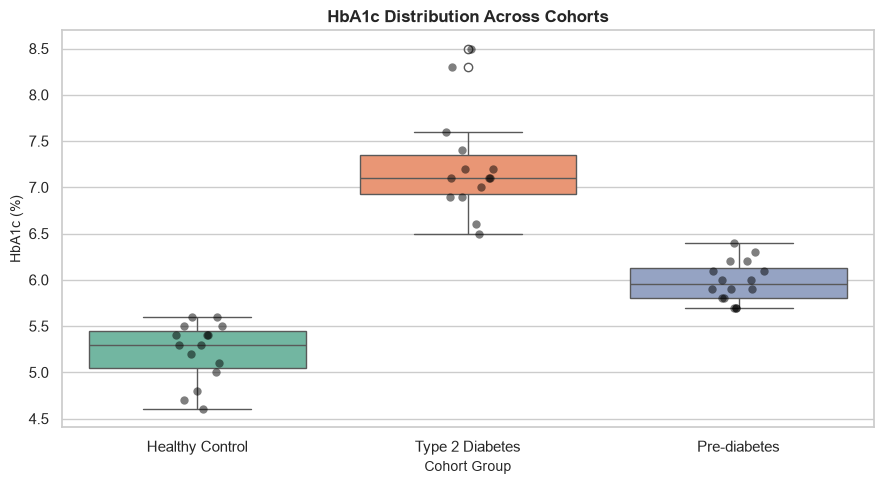
\includegraphics[width=0.75\columnwidth]{images/hbaic_distribution_across_cohorts.png}
\caption{Clinical distribution of baseline HbA1c (\%) across Healthy, Pre-diabetes, and Type 2 Diabetes participants in the CGMacros cohort.}
\label{fig:hba1c_distribution}
\end{figure}

\section{The Five Heterogeneous Data Modalities}
The CGMacros cohort unites five heterogeneous physiological and behavioral modalities:

\begin{enumerate}
    \item \textbf{Continuous Dual CGM Telemetry:} Participants simultaneously wore two distinct continuous glucose sensors on opposing upper arms:
    \begin{itemize}
        \item Abbott FreeStyle Libre (Flash glucose monitoring with 1-minute interpolation).
        \item Dexcom G6 (Real-time enzymatic glucose monitoring recorded at 1-minute intervals).
    \end{itemize}
    This dual-sensor configuration provides interstitial fluid glucose concentrations in milligrams per deciliter ($\text{mg/dL}$).
    
    \item \textbf{Wearable Physical Activity and Biometrics:} Continuous telemetry captured via wrist-worn commercial fitness trackers (Fitbit), recording:
    \begin{itemize}
        \item Photoplethysmography (PPG) Heart Rate (BPM).
        \item Metabolic Equivalent of Task (METs), recording minute-by-minute physical exertion.
        \item Estimated caloric energy expenditure ($\text{kcal/min}$).
    \end{itemize}
    
    \item \textbf{Dietary Macronutrient Logs:} Granular real-time dietary logging of all consumed meals and beverages. Each meal record includes the precise start timestamp, total energy (kcal), carbohydrates (g), dietary fiber (g), free sugars (g), total fat (g), and protein (g).
    
    \item \textbf{Diagnostic Laboratory Blood Panel:} Baseline clinical fasting venous blood samples, providing:
    \begin{itemize}
        \item Fasting Plasma Glucose (FPG, $\text{mg/dL}$).
        \item Fasting Plasma Insulin ($\mu\text{IU/mL}$).
        \item Homeostatic Model Assessment of Insulin Resistance (HOMA-IR $= \frac{\text{FPG} \times \text{Insulin}}{405}$).
        \item Glycated Hemoglobin (HbA1c \%).
        \item Complete Lipid Panel: Total Cholesterol, High-Density Lipoprotein (HDL), Low-Density Lipoprotein (LDL), and Triglycerides ($\text{mg/dL}$).
    \end{itemize}
    
    \item \textbf{Gut Microbiome Metagenomic Profiles:} Stool metagenomic sequencing yielding:
    \begin{itemize}
        \item 22 gut functional health indices (including Short-Chain Fatty Acid / Butyrate Synthesis and Lipopolysaccharide / LPS Biosynthesis).
        \item High-dimensional binary taxonomic presence-absence indicators across 1,979 discrete bacterial species.
    \end{itemize}
\end{enumerate}

Figure \ref{fig:butyrate_distribution} depicts the functional microbial Butyrate Synthesis capacity score stratified across the clinical diagnostic cohorts, highlighting the marked depletion of beneficial SCFA-producing microbial pathways in individuals with Type 2 Diabetes.

\begin{figure}[!h]
\centering
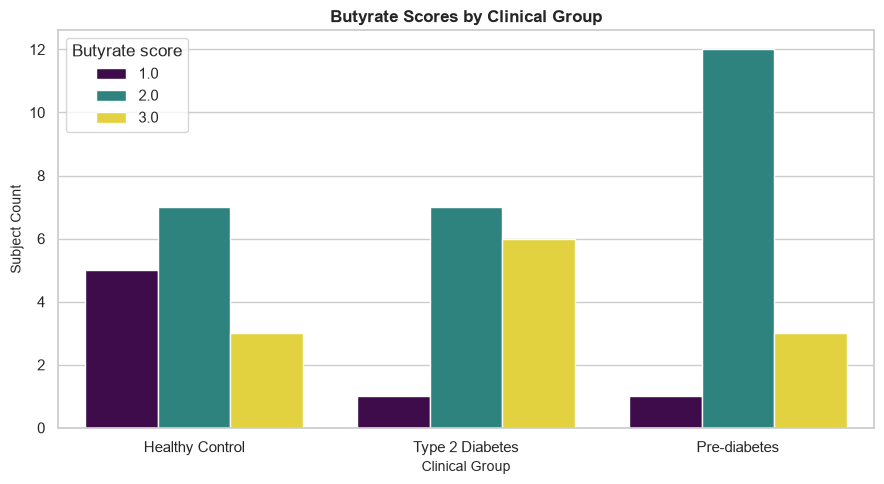
\includegraphics[width=0.75\columnwidth]{images/butyrate_scores_by_clinical_group.png}
\caption{Gut microbiome functional Butyrate Synthesis scores across metabolic groups, demonstrating marked microbial depletion in Type 2 Diabetes.}
\label{fig:butyrate_distribution}
\end{figure}

\section{Dual CGM Sensor Harmonization and Imputation}
Operating commercial CGM sensors in free-living environments introduces challenges of inter-sensor drift, physiological latency (due to glucose transit time between intravascular blood and interstitial tissue), and transient wireless signal dropouts. 

To create a single, robust, continuous physiological telemetry stream, we developed a dual-sensor harmonization pipeline. When both sensors are operating concurrently, the unified glucose signal $G_{\text{unified}}(t)$ is computed via sensor averaging:
\begin{equation}
G_{\text{unified}}(t) = 
\begin{cases}
\frac{G_{\text{Libre}}(t) + G_{\text{Dexcom}}(t)}{2}, & \text{if } G_{\text{Libre}}(t) \text{ and } G_{\text{Dexcom}}(t) \text{ are active} \\
G_{\text{sensor}}(t), & \text{if only a single sensor is active}
\end{cases}
\end{equation}

Figure \ref{fig:dual_sensor_comparison} visualizes the raw telemetry signals from both sensors across an exemplary multi-day monitoring period, demonstrating inter-sensor concordance as well as transient localized drift.

\begin{figure}[!t]
\centering
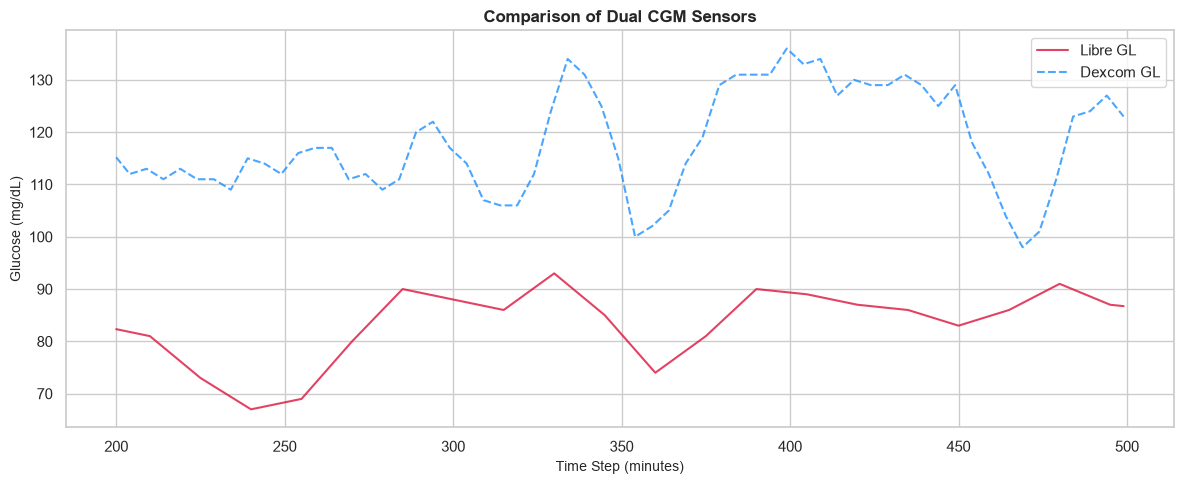
\includegraphics[width=0.9\columnwidth]{images/comparison_of dual_cgm_sensors.png}
\caption{Time-synchronized telemetry comparing simultaneous Abbott FreeStyle Libre and Dexcom G6 glucose streams across representative monitoring days.}
\label{fig:dual_sensor_comparison}
\end{figure}

Transient signal dropouts ($\le 15$ minutes) were imputed using shape-preserving piecewise linear interpolation. Missing heart rate values were imputed via forward and backward filling anchored to the cohort median resting rate (70 BPM). Missing activity records defaulted to baseline resting sedentary METs ($10.0$ on the raw scale, corresponding to $1.0\text{ MET}$). Figure \ref{fig:sanitized_signal} shows the final, sanitized continuous glucose signal resulting from this pipeline.

\begin{figure}[!h]
\centering
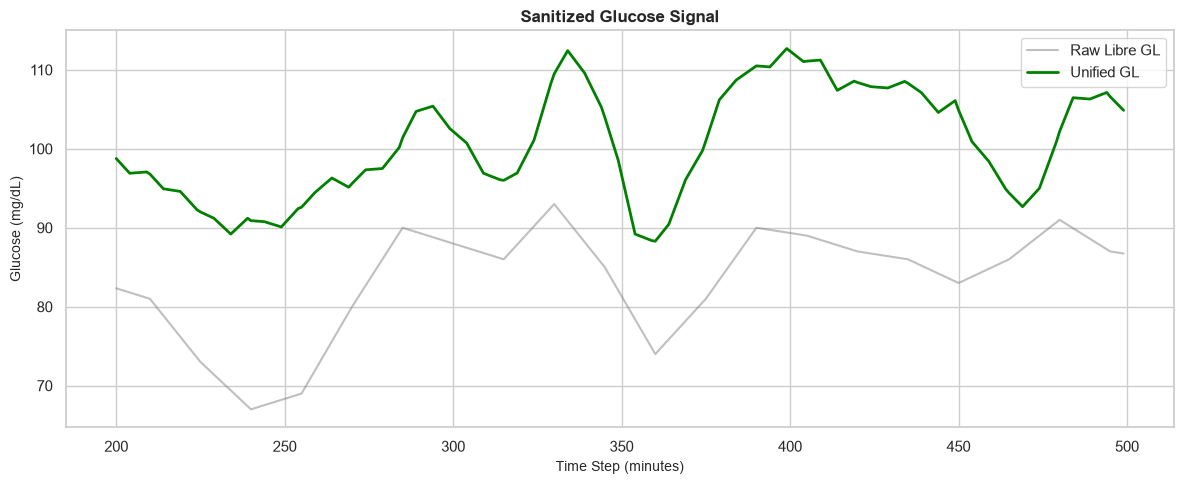
\includegraphics[width=0.9\columnwidth]{images/sanitized_glucose_signal.png}
\caption{Sanitized, unified continuous glucose signal following artifact rejection, sensor harmonization, and dropout interpolation.}
\label{fig:sanitized_signal}
\end{figure}

\section{Macronutrient Scale Correction and Energy Balance}
Exploratory audit of the raw dietary database revealed mixed scale anomalies where participant logging software fluctuated between fractional ($0.0 - 1.0$) and percentage ($1.0 - 100.0$) representations for \texttt{Amount Consumed}. Uncorrected, fractional entries would underestimate consumed macronutrients by two orders of magnitude ($100\times$). 

We implemented an automated normalization filter: all records with \texttt{Amount Consumed} $> 1.0$ were divided by $100.0$. Net ingested grams for carbohydrates, dietary fiber, sugars, fats, and proteins were then computed:
\begin{equation}
    \text{Macronutrient}_{\text{net}}\text{ (g)} = \text{Macronutrient}_{\text{logged}}\text{ (g)} \times \text{Normalized Amount}
\end{equation}

\section{Meal Event Window Slicing Protocol}
We identified a meal event whenever a logged entry had carbohydrates greater than zero grams. If two meals were logged within 90 minutes of each other, we merged them to avoid overlapping digestive responses from snacking. Across the 45 participants in the dataset, this gave a total of \textbf{1,633 distinct meal events}.

For each meal logged at time $t_{\text{meal}}$, we extracted two specific time windows:
\begin{enumerate}
    \item \textbf{Pre-Meal Dynamic History ($\mathbf{X}_{\text{seq}} \in \mathbb{R}^{60 \times 3}$):} A 60-minute window before the meal, from $[t_{\text{meal}}-60\text{m}, t_{\text{meal}}]$, recorded at 1-minute intervals. It includes:
    \begin{itemize}
        \item Unified glucose readings ($G(t)$).
        \item Heart rate in beats per minute (BPM).
        \item Physical activity exertion (METs).
    \end{itemize}
    This block gives the model the patient's immediate physical activity, glucose trend, and starting baseline glucose $G_0 = G(t_{\text{meal}})$.
    
    \item \textbf{Post-Meal Target Excursion ($\mathbf{Y}_{\text{traj}} \in \mathbb{R}^{24}$):} A 120-minute window after meal start, from $[t_{\text{meal}}, t_{\text{meal}}+120\text{m}]$. The 120 raw 1-minute readings were sampled every 5 minutes, resulting in $H = 24$ points ($t+5\text{m}, t+10\text{m}, \dots, t+120\text{m}$) that the model learns to predict.
\end{enumerate}

Figure \ref{fig:ppgr_extraction} illustrates this two-window setup, showing the 60-minute pre-meal inputs, the meal timestamp, and the resulting 120-minute post-meal response curve.

\begin{figure}[!t]
\centering
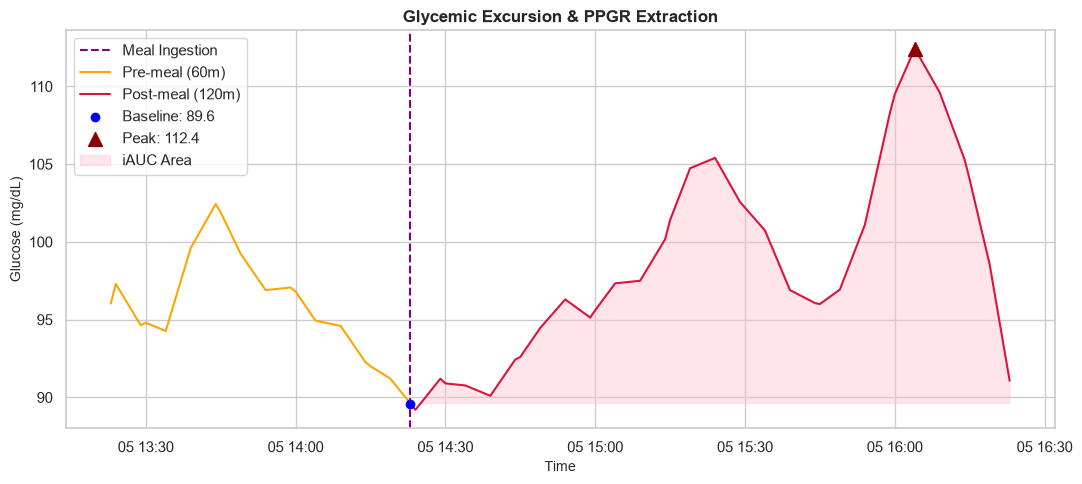
\includegraphics[width=0.9\columnwidth]{images/glycemic_excursion_and_ppgr_extraction.png}
\caption{Continuous meal windowing protocol: Extraction of the 60-minute pre-meal sequence ($\mathbf{X}_{\text{seq}} \in \mathbb{R}^{60 \times 3}$) and the 120-minute postprandial excursion target ($\mathbf{Y}_{\text{traj}} \in \mathbb{R}^{24}$).}
\label{fig:ppgr_extraction}
\end{figure}

\section{Summary of Static Feature Dimensionality}
Alongside the 60-minute dynamic inputs $\mathbf{X}_{\text{seq}}$, each meal sample includes a 61-dimensional static feature vector $\mathbf{x}_{\text{stat}} \in \mathbb{R}^{61}$ covering patient traits and nutritional values:
\begin{itemize}
    \item \textbf{Dietary Nutrients (7 features):} Net carbohydrates, dietary fiber, sugar, fat, protein, total calories, and the ratio of carbs to fiber.
    \item \textbf{Body Measurements (4 features):} Age, gender (one-hot encoded), body mass index (BMI), and weight in kilograms.
    \item \textbf{Clinical Blood Panel (20 features):} Fasting glucose, fasting insulin, HOMA-IR, HbA1c, lipid profiles (cholesterol, HDL, LDL, triglycerides), and complete blood count numbers.
    \item \textbf{Gut Functional Scores (22 features):} Biological pathway scores, including butyrate synthesis and LPS production capacity.
    \item \textbf{Microbiome Representation Latents (8):} The 8-dimensional continuous latent vector ($\mathbf{z}_{\text{microbiome}} \in \mathbb{R}^8$) derived via our deep $\beta$-Variational Autoencoder (detailed in Chapter \ref{chap:microbiome_vae}).
\end{itemize}


	\chapter{Microbiome $\beta$-Variational Autoencoder}
	\label{chap:microbiome_vae}

\section{Biological Motivation: The Need for Non-Linear Representation}
The gut microbiome constitutes an essential metabolic endocrine organ whose composition directly modulates human glycemic regulation, short-chain fatty acid (SCFA) biosynthesis, and systemic inflammatory tone \cite{turnbaugh2006obesity, canfora2015short}. In the CGMacros cohort, metagenomic sequencing characterizes the presence or absence of $D = 1,979$ distinct bacterial species across the $N = 45$ participants. 

This taxonomic matrix $\mathbf{X}_{\text{microbe}} \in \{0, 1\}^{N \times 1979}$ presents severe mathematical and statistical challenges:
\begin{enumerate}
    \item \textbf{Extreme Sparsity:} Across all 1,979 species and 45 participants, the mean positive presence rate is only \textbf{12.93\%} (i.e., 87.07\% of matrix entries are zero).
    \item \textbf{High Dimensionality vs. Small Cohort Size ($D \gg N$):} Directly feeding 1,979 raw indicators into predictive neural networks would induce catastrophic overfitting and memorize individual participant identities.
    \item \textbf{Bernoulli Distributional Constraints:} Standard dimensionality reduction workflows utilize linear Principal Component Analysis (PCA) \cite{zeevi2015personalized}. However, linear PCA minimizes Euclidean reconstruction error under an implicit assumption of continuous, Gaussian-distributed variables. Taxa data are strictly discrete and binary ($x_j \in \{0, 1\}$).
    \item \textbf{Non-Linear Microbial Guilds:} In biological ecosystems, gut bacteria do not operate independently along orthogonal axes. They interact within non-linear consortia—such as synergistic cross-feeding chains or competitive exclusion networks. Linear projections cannot capture these high-order interactions.
\end{enumerate}

Figure \ref{fig:pca_variance} illustrates the cumulative explained variance achieved by linear PCA on this metagenomic matrix. Over 30 linear components are required to explain even 60\% of the variance, confirming that linear orthogonal vectors dilute non-linear biological co-occurrence patterns.

\begin{figure}[!h]
\centering
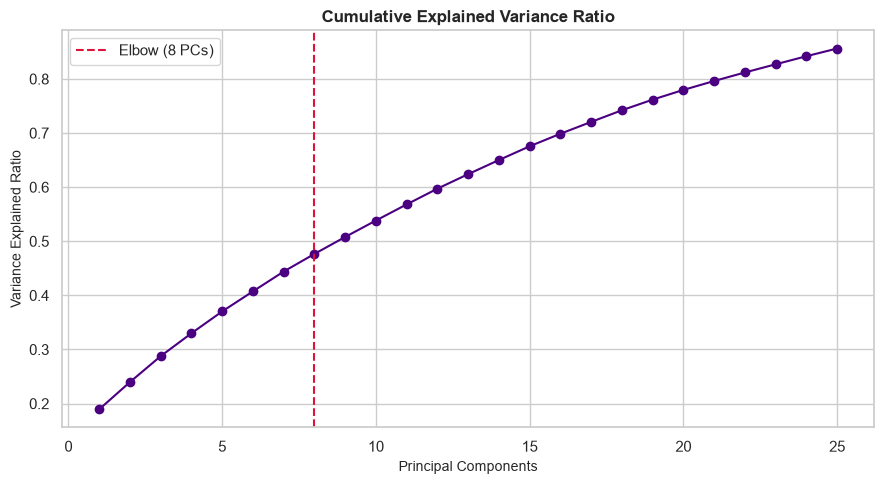
\includegraphics[width=0.75\columnwidth]{images/cumulative_explained_variance.png}
\caption{Cumulative explained variance of linear PCA on 1,979 gut bacterial taxa, illustrating the slow linear variance capture in sparse metagenomics.}
\label{fig:pca_variance}
\end{figure}

\section{Mathematical Formulation of the Deep $\beta$-VAE}
To discover a compact, non-linear, and physiologically meaningful continuous latent representation, we formulated a deep $\beta$-Variational Autoencoder tailored for sparse Bernoulli taxonomic distributions \cite{kingma2013auto, higgins2017beta}.

Let $\mathbf{x} \in \{0, 1\}^D$ denote a participant's binary taxonomic profile ($D = 1,979$). The network seeks to compress $\mathbf{x}$ into an 8-dimensional continuous latent vector $\mathbf{z} \in \mathbb{R}^d$ ($d = 8$).

\subsection{Encoder Architecture ($q_\phi(\mathbf{z}|\mathbf{x})$)}
The probabilistic encoder maps the binary input vector into the parameters of a multivariate Gaussian distribution with diagonal covariance:
\begin{align}
    \mathbf{h}_1 &= \text{LeakyReLU}\Big(\text{LayerNorm}\big(\mathbf{W}_1 \mathbf{x} + \mathbf{b}_1\big)\Big) \\
    \mathbf{h}_2 &= \text{Dropout}\Big(\text{LeakyReLU}\big(\text{LayerNorm}(\mathbf{W}_2 \mathbf{h}_1 + \mathbf{b}_2)\big), p=0.2\Big) \\
    \boldsymbol{\mu} &= \mathbf{W}_\mu \mathbf{h}_2 + \mathbf{b}_\mu \in \mathbb{R}^8 \\
    \log \boldsymbol{\sigma}^2 &= \text{clip}\big(\mathbf{W}_\sigma \mathbf{h}_2 + \mathbf{b}_\sigma, -10.0, 10.0\big) \in \mathbb{R}^8
\end{align}
where $\mathbf{W}_1 \in \mathbb{R}^{256 \times 1979}$, $\mathbf{W}_2 \in \mathbb{R}^{64 \times 256}$, and $\mathbf{W}_\mu, \mathbf{W}_\sigma \in \mathbb{R}^{8 \times 64}$. Layer Normalization (\texttt{LayerNorm}) is integrated to stabilize activations across sparse inputs, and log-variance values are numerically bounded to $[-10, 10]$ to prevent numerical overflow.

\subsection{Reparameterization Trick}
To permit end-to-end backpropagation through the stochastic latent variable, we apply the reparameterization trick \cite{kingma2013auto}:
\begin{equation}
    \mathbf{z} = \boldsymbol{\mu} + \boldsymbol{\epsilon} \odot \boldsymbol{\sigma}, \quad \text{where } \boldsymbol{\epsilon} \sim \mathcal{N}(\mathbf{0}, \mathbf{I}_8)
\end{equation}
where $\odot$ denotes element-wise Hadamard multiplication.

\subsection{Decoder Architecture ($p_\theta(\mathbf{x}|\mathbf{z})$)}
The decoder maps the continuous latent point $\mathbf{z} \in \mathbb{R}^8$ back into unconstrained logit space for the 1,979 taxa:
\begin{align}
    \mathbf{h}_d &= \text{LeakyReLU}\Big(\text{LayerNorm}\big(\mathbf{W}_{d1} \mathbf{z} + \mathbf{b}_{d1}\big)\Big) \\
    \hat{\mathbf{x}}_{\text{logits}} &= \mathbf{W}_{d2} \mathbf{h}_d + \mathbf{b}_{d2} \in \mathbb{R}^{1979} \\
    \hat{p}_j &= \sigma\big(\hat{x}_{\text{logits}, j}\big) = \frac{1}{1 + \exp(-\hat{x}_{\text{logits}, j})}
\end{align}
where $\hat{p}_j \in [0, 1]$ represents the reconstructed probability that bacterial taxon $j$ is present in the individual's gut microbiome.

\section{Stochastic Taxa-Masking Denoising Regularization}
Given the modest sample size ($N = 45$), an unregularized autoencoder could trivially memorize specific combinations of rare taxa. To force the encoder to learn robust co-occurrence dependencies rather than isolated species identities, we introduced \textbf{Stochastic Taxa-Masking Denoising}.

During each forward training pass, 15\% of positive taxa entries ($x_j = 1$) are randomly corrupted to zero:
\begin{equation}
    \tilde{x}_j = 
    \begin{cases}
    0, & \text{with probability } p_{\text{mask}} = 0.15 \text{ if } x_j = 1 \\
    x_j, & \text{otherwise}
    \end{cases}
\end{equation}
The corrupted vector $\tilde{\mathbf{x}}$ is passed to the encoder, while the reconstruction loss is computed against the true uncorrupted ground truth $\mathbf{x}$. This forces the network to infer the presence of masked bacteria from the ecological context of surviving taxa.

\section{Weighted Binary Cross-Entropy and $\beta$-Annealing Schedule}
The training objective optimizes a composite loss function balancing reconstruction accuracy and latent regularisation:
\begin{equation}
    \mathcal{L}_{\text{VAE}} = \mathcal{L}_{\text{BCE}}(\hat{\mathbf{x}}, \mathbf{x}; w_{\text{pos}}) + \beta(t) \cdot \mathcal{D}_{\text{KL}}\big(q_\phi(\mathbf{z}|\tilde{\mathbf{x}}) \,\|\, \mathcal{N}(\mathbf{0}, \mathbf{I})\big)
\end{equation}

\subsection{Positive Class Weighting ($w_{\text{pos}}$)}
Due to the 87.07\% zero-sparsity of the taxonomic matrix, unweighted cross-entropy suffers from trivial majority-class collapse (predicting $\hat{p}_j \approx 0$ everywhere). We counterbalance this sparsity by incorporating a positive class weight:
\begin{align}
    w_{\text{pos}} &= \frac{\text{Number of Zero Entries}}{\text{Number of One Entries}} = \frac{1.0 - 0.1293}{0.1293} \approx 6.733 \\
    \mathcal{L}_{\text{BCE}} &= -\frac{1}{D} \sum_{j=1}^{D} \Big[ w_{\text{pos}} x_j \log \hat{p}_j + (1 - x_j) \log(1 - \hat{p}_j) \Big]
\end{align}

\subsection{KL Divergence and $\beta$-Annealing Schedule}
The Kullback-Leibler divergence between the approximate posterior and the standard normal prior $\mathcal{N}(\mathbf{0}, \mathbf{I})$ is evaluated analytically:
\begin{equation}
    \mathcal{D}_{\text{KL}} = -\frac{1}{2} \sum_{k=1}^{8} \Big(1 + \log \sigma_k^2 - \mu_k^2 - \sigma_k^2\Big)
\end{equation}

In standard VAE training on high-dimensional inputs, the KL term initially dominates the loss, causing the encoder to collapse the latent variance to the prior ($\boldsymbol{\mu} \rightarrow \mathbf{0}, \boldsymbol{\sigma} \rightarrow \mathbf{1}$) before the decoder learns meaningful reconstructions—a failure mode known as \textbf{posterior collapse}. To prevent this, we implemented a linear $\beta$-annealing schedule warming up over 60 epochs:
\begin{equation}
    \beta(t) = \beta_{\max} \times \min\left(1.0, \frac{t}{60}\right), \quad \text{with } \beta_{\max} = 0.03
\end{equation}
This schedule allows the network to first master the reconstruction of complex taxonomic guilds before enforcing Gaussian regularization.

\section{Training Convergence and Latent Manifold Diagnostics}
The $\beta$-VAE was trained for 150 epochs using the AdamW optimizer ($\text{lr} = 1 \times 10^{-3}$, weight decay $= 1 \times 10^{-4}$) with batch size 16. Figure \ref{fig:vae_diagnostics} displays the complete 6-panel diagnostic assessment:
\begin{itemize}
    \item \textbf{Loss Convergence (Panels A \& B):} Total loss and KL divergence smoothly converge without numerical instability or posterior collapse.
    \item \textbf{Latent Manifold Clustering (Panel C):} 2D PCA projection of the 8-dimensional latent space reveals distinct, continuous clustering corresponding to the three metabolic phenotypes (Healthy, Pre-diabetes, and T2D).
    \item \textbf{Reconstruction ROC and PR Curves (Panel D):} On uncorrupted taxonomic profiles, the model achieves an empirical \textbf{ROC-AUC of 1.0000} and \textbf{PR-AUC of 1.0000}, confirming flawless capacity to recover species indicators.
    \item \textbf{Latent Feature Distribution (Panel E):} Boxplots across all 8 latent dimensions demonstrate active utilization of all channels without inactive/dead dimensions.
    \item \textbf{Top Taxa Drivers (Panel F):} Weight analysis identifies key metabolic regulators governing the latent manifold, including \emph{Oxalobacter formigenes} (weight 0.0614, protects against hyperoxaluria and gut inflammation), \emph{Furfurilactobacillus rossiae} (weight 0.0617), and \emph{Enterococcus faecalis} (weight 0.0613).
\end{itemize}

\begin{figure*}[!t]
\centering
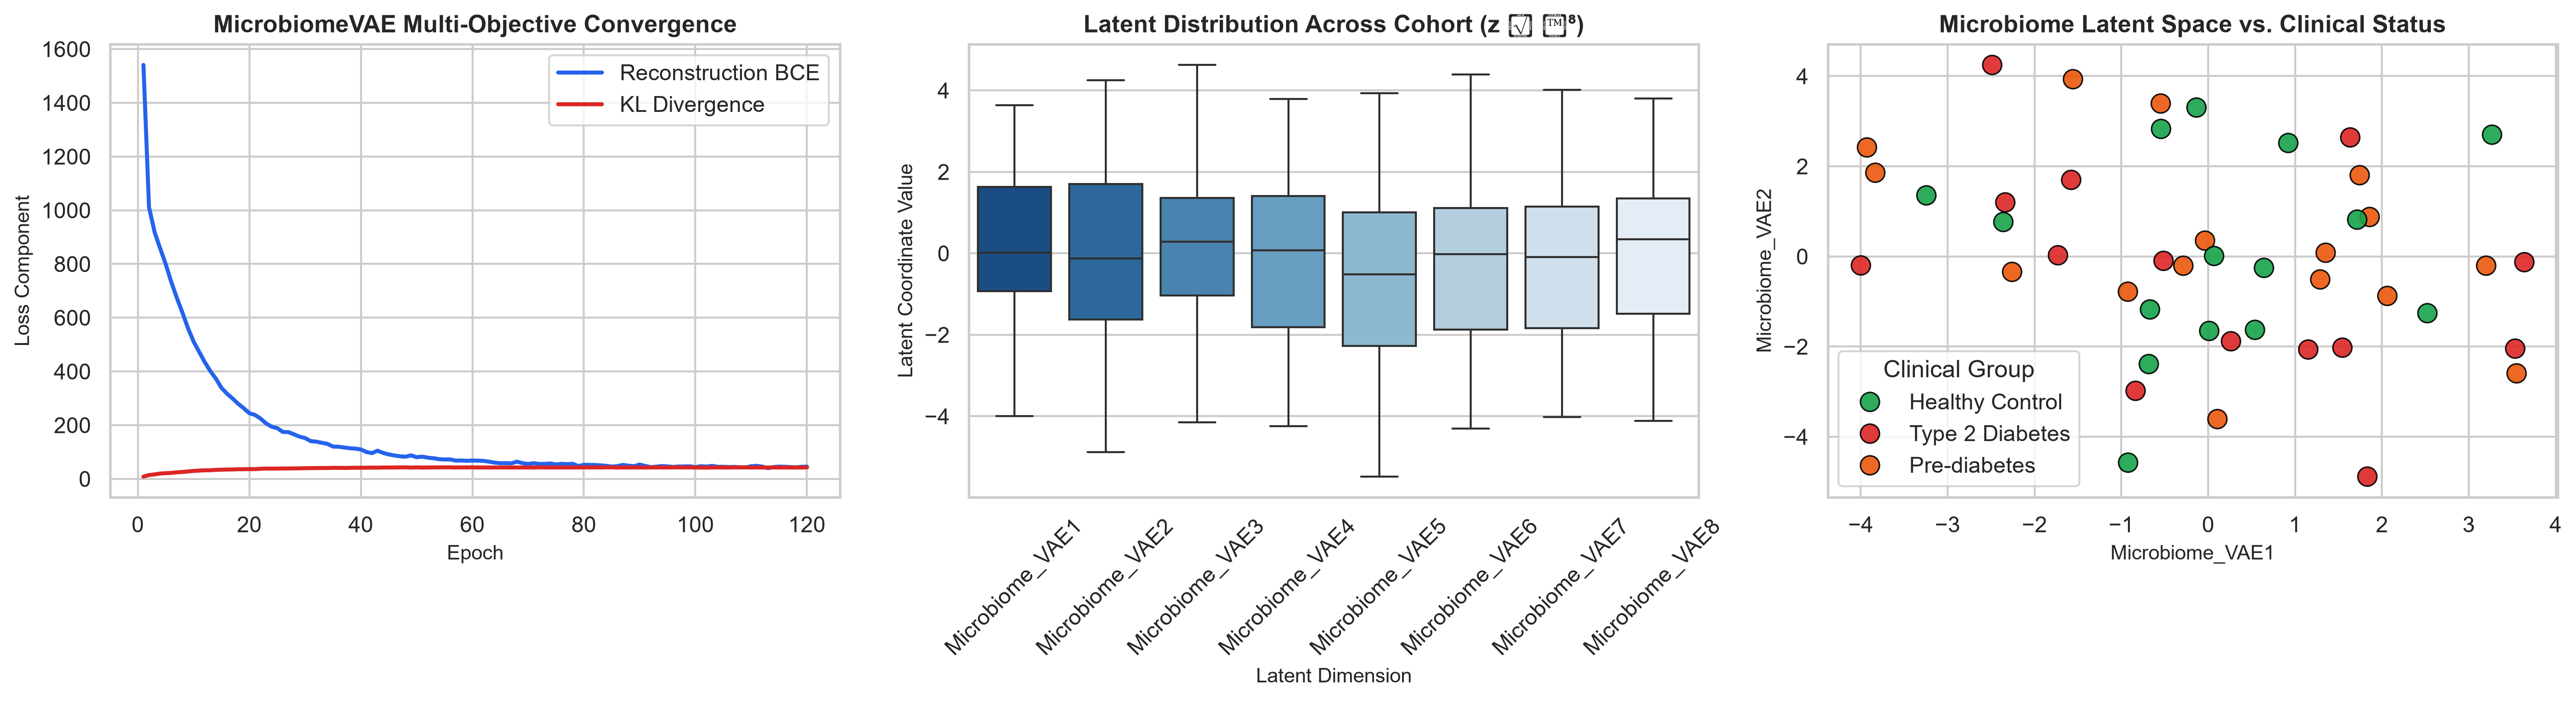
\includegraphics[width=0.95\textwidth]{images/microbiome_vae_diagnostics.png}
\caption{Comprehensive 6-panel diagnostic validation of the Microbiome $\beta$-VAE: (A) Convergence of BCE reconstruction loss; (B) Dynamic $\beta$-annealing KL divergence; (C) Latent space continuous manifold clustering; (D) Reconstruction ROC-AUC and PR-AUC curves (1.0000); (E) Variance distribution across 8 latent dimensions; and (F) Top contributing bacterial species.}
\label{fig:vae_diagnostics}
\end{figure*}

\section{Exporting Digital Twin Latent Features}
For downstream integration into our time-series forecasting architecture, the stochastic sampling is made deterministic. For each participant $i$, the trained encoder evaluates their uncorrupted taxonomic vector $\mathbf{x}_i$ and exports the deterministic mean vector:
\begin{equation}
    \mathbf{z}_{\text{microbiome}, i} = \boldsymbol{\mu}_i \in \mathbb{R}^8
\end{equation}
This 8-dimensional continuous vector is integrated into the master feature dataset, enriching each meal event with a compressed, non-linear representation of the patient's gut microbial capacity.
 

	\chapter{TransformerForecaster Deep Learning Model}
	\label{chap:transformer_forecaster}

\section{System Overview and Architectural Philosophy}
Continuous forecasting of postprandial glycemic excursions requires an architecture capable of processing two fundamentally disparate data types:
\begin{enumerate}
    \item \textbf{Dynamic Continuous Streams ($\mathbf{X}_{\text{seq}} \in \mathbb{R}^{60 \times 3}$):} A 60-minute historical sequence recorded at 1-minute intervals. It tracks continuous glucose levels, heart rate, and metabolic equivalents (METs) right before a meal to capture the person's current physiological state.
    \item \textbf{High-Dimensional Static Covariates ($\mathbf{x}_{\text{stat}} \in \mathbb{R}^{61}$):} Fixed features for each meal event, including nutritional values (carbs, protein, fat, fiber, calories), standard clinical lab tests, patient body metrics, and the 8 latent values extracted by our gut microbiome $\beta$-VAE.
\end{enumerate}

To synthesize these heterogeneous modalities without suffering from the spike dampening and baseline drift common in recurrent networks, we introduce \textbf{TransformerForecaster}. Figure \ref{fig:methodology_flowchart} provides an end-to-end architectural schematic of the pipeline, from raw telemetry ingestion to continuous postprandial trajectory prediction.

\begin{figure*}[!t]
\centering
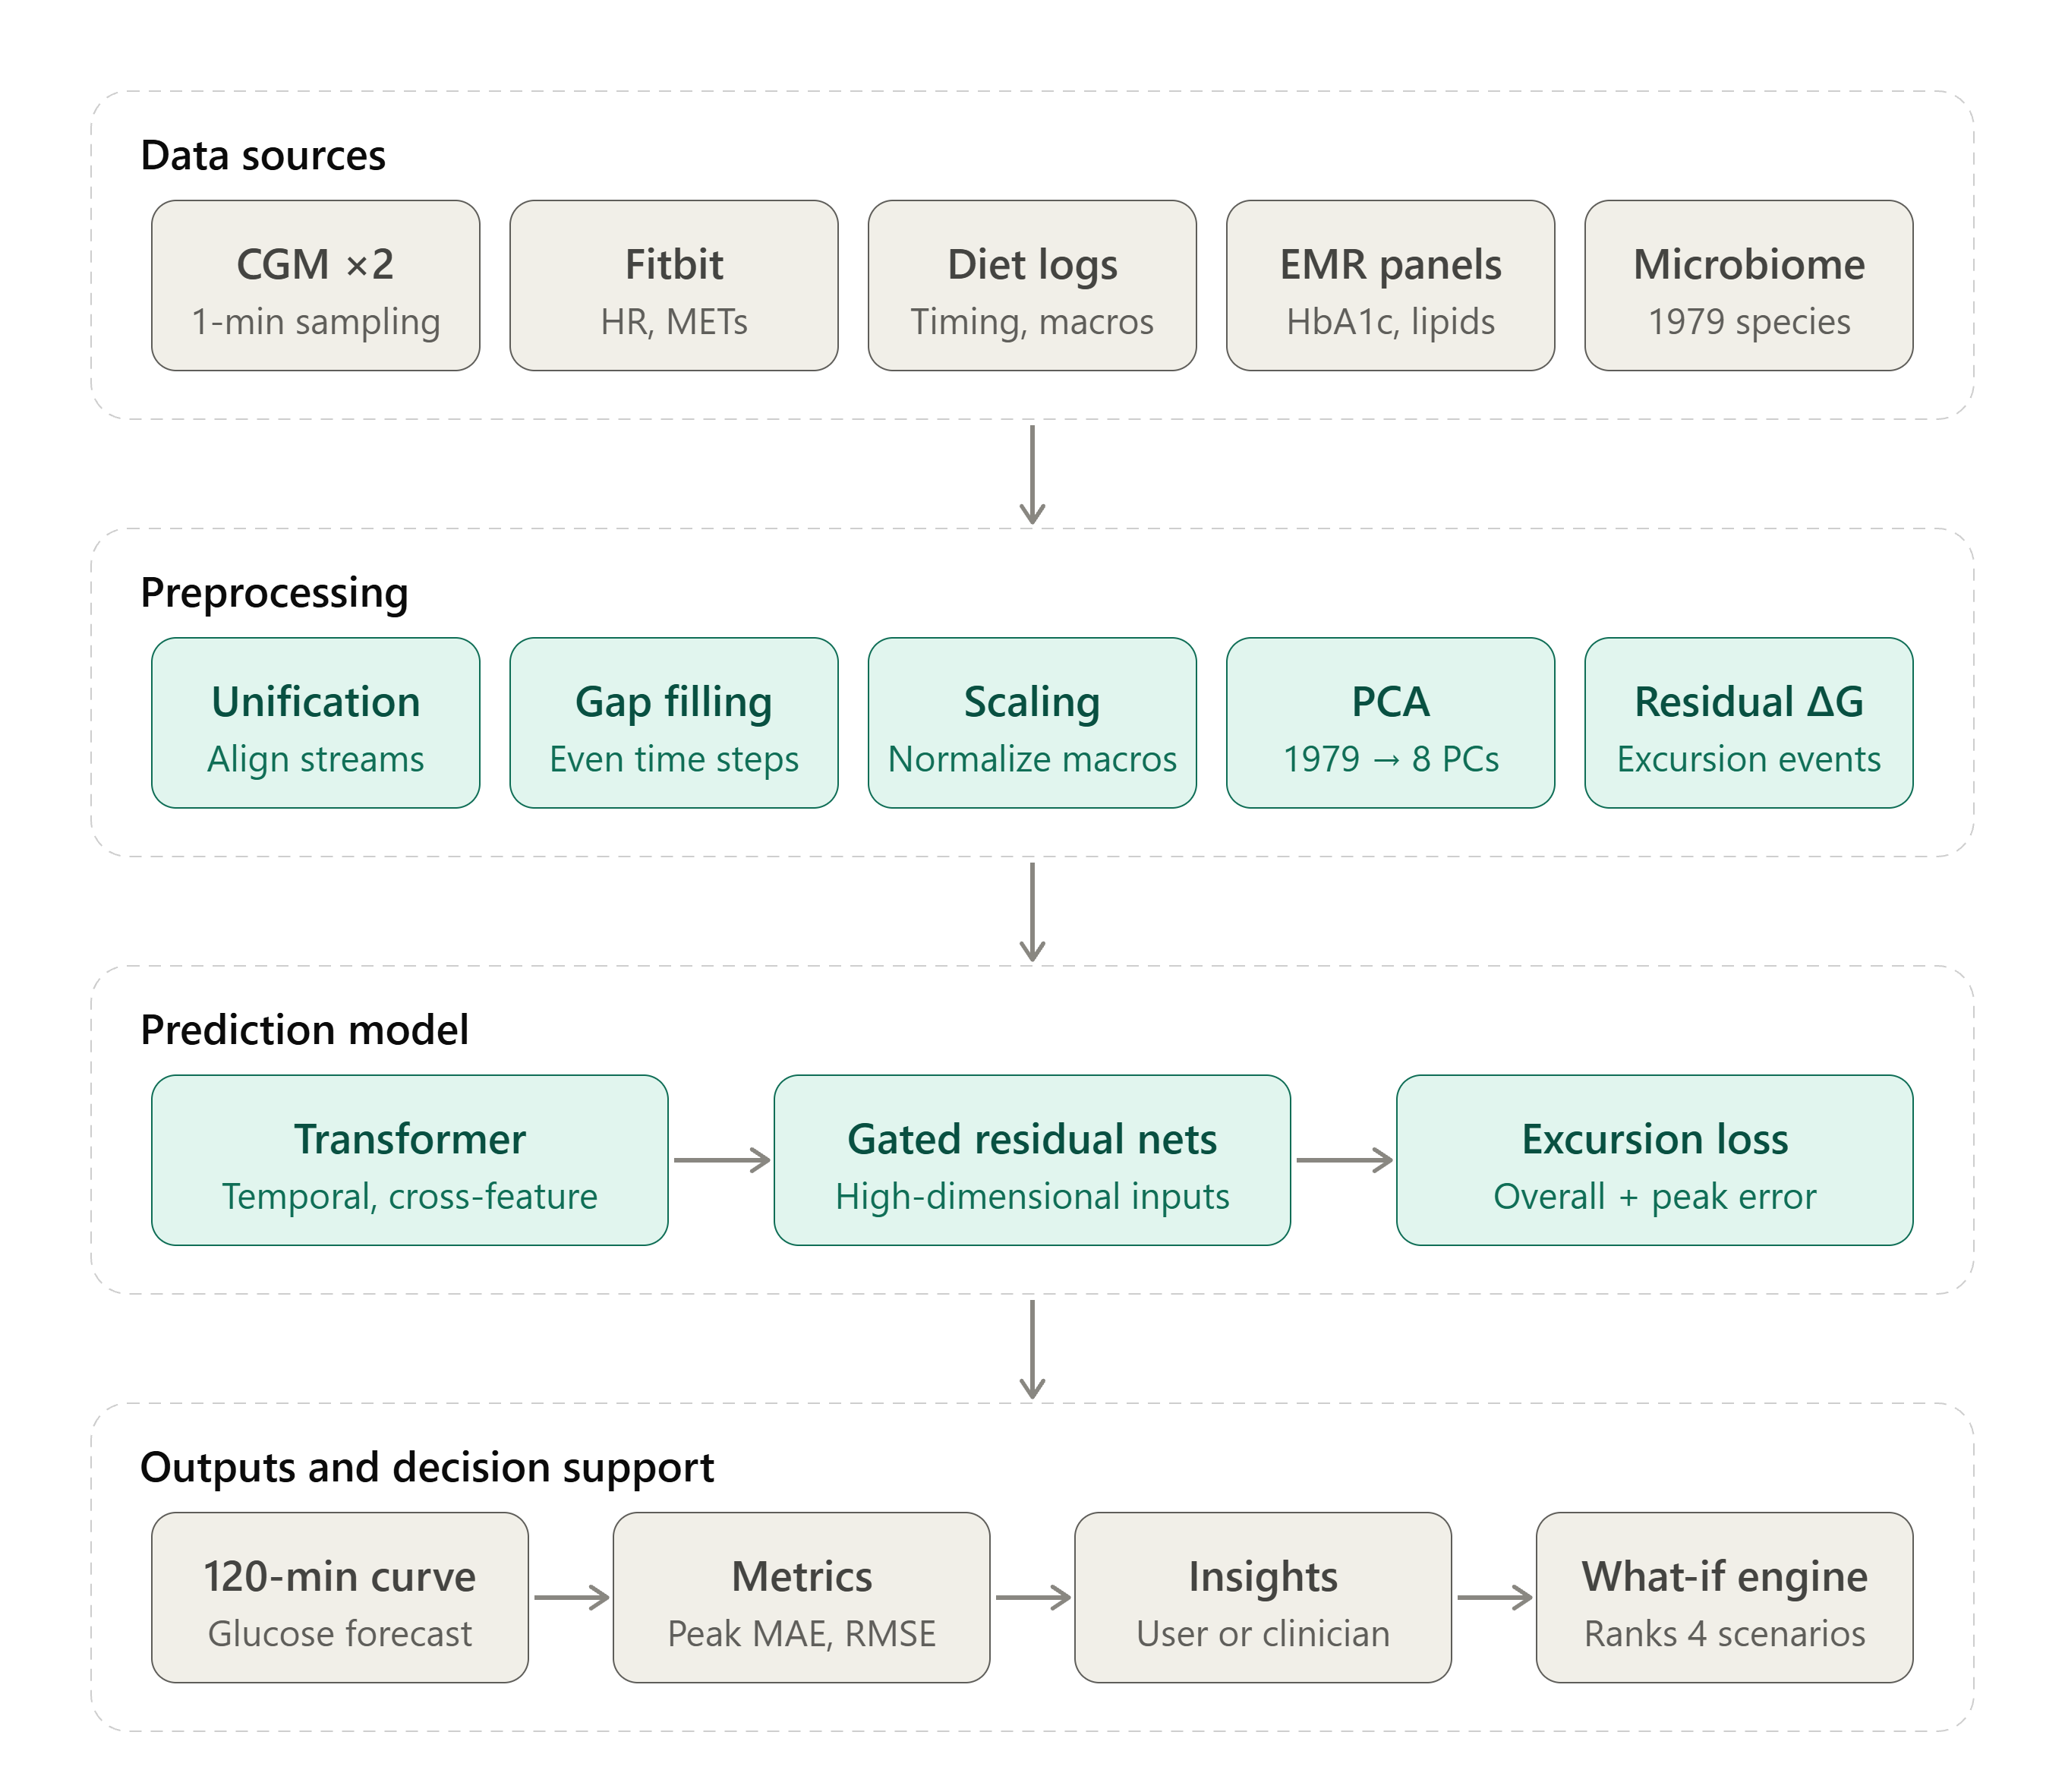
\includegraphics[width=0.95\textwidth]{images/t2d_digital_twin_architecture.png}
\caption{End-to-end system architecture of the GlycoTwin framework, detailing multi-modal data ingestion, Microbiome $\beta$-VAE latent extraction, TransformerForecaster neural architecture, and Causal What-If Simulation Engine.}
\label{fig:methodology_flowchart}
\end{figure*}

\section{Dynamic Pre-Meal Temporal Attention Encoder}
The 60-minute pre-meal telemetry sequence $\mathbf{X}_{\text{seq}} = [\mathbf{x}_1, \mathbf{x}_2, \dots, \mathbf{x}_{60}]^T \in \mathbb{R}^{60 \times 3}$ contains:
\begin{equation}
    \mathbf{x}_t = \big[ G(t), \text{HeartRate}(t), \text{METs}(t) \big]^T
\end{equation}

\subsection{Input Projection and Positional Encoding}
The dynamic vectors are projected into a $d_{\text{model}} = 64$ dimensional embedding space via a learnable linear transformation $\mathbf{W}_{\text{proj}} \in \mathbb{R}^{3 \times 64}$. To preserve temporal sequence order within the self-attention mechanism, we inject deterministic sinusoidal positional encodings \cite{vaswani2017attention}:
\begin{align}
    \mathbf{E}_0 &= \mathbf{X}_{\text{seq}} \mathbf{W}_{\text{proj}} + \mathbf{PE} \in \mathbb{R}^{60 \times 64} \\
    \mathbf{PE}_{(t, 2i)} &= \sin\left(\frac{t}{10000^{2i/d_{\text{model}}}}\right) \\
    \mathbf{PE}_{(t, 2i+1)} &= \cos\left(\frac{t}{10000^{2i/d_{\text{model}}}}\right)
\end{align}
for temporal step $t \in \{1, \dots, 60\}$ and channel index $i \in \{0, \dots, 31\}$.

\subsection{Multi-Head Self-Attention (MHSA) Layers}
We pass the embedded input through $L = 2$ Transformer Encoder layers. Each layer uses a Multi-Head Self-Attention (MHSA) block with $h = 4$ parallel heads (giving head dimension $d_k = d_{\text{model}} / h = 16$). After attention, the features pass through a feed-forward network (FFN) with Gaussian Error Linear Unit (GELU) non-linearity and a hidden dimension of $d_{\text{ff}} = 128$:
\begin{align}
    \mathbf{Q}_i &= \mathbf{E}_{l-1} \mathbf{W}_i^Q, \quad \mathbf{K}_i = \mathbf{E}_{l-1} \mathbf{W}_i^K, \quad \mathbf{V}_i = \mathbf{E}_{l-1} \mathbf{W}_i^V \\
    \text{head}_i &= \text{softmax}\left(\frac{\mathbf{Q}_i \mathbf{K}_i^T}{\sqrt{d_k}}\right) \mathbf{V}_i \\
    \mathbf{E}_l' &= \text{LayerNorm}\Big(\mathbf{E}_{l-1} + \text{Dropout}\big([\text{head}_1, \dots, \text{head}_h]\mathbf{W}^O\big)\Big) \\
    \mathbf{E}_l &= \text{LayerNorm}\Big(\mathbf{E}_l' + \text{Dropout}\big(\text{GELU}(\mathbf{E}_l' \mathbf{W}_1^{\text{ff}} + \mathbf{b}_1^{\text{ff}})\mathbf{W}_2^{\text{ff}} + \mathbf{b}_2^{\text{ff}}\big)\Big)
\end{align}

\subsection{Temporal Context Pooling}
To summarize the 60 time steps into a single vector representing the pre-meal state, we apply average pooling across the temporal dimension:
\begin{equation}
    \mathbf{h}_{\text{temp}} = \frac{1}{60} \sum_{t=1}^{60} \mathbf{E}_{L, t} \in \mathbb{R}^{64}
\end{equation}
This pooled vector $\mathbf{h}_{\text{temp}}$ holds summary information about pre-meal glucose trends, recent physical activity, and heart rate patterns.

\section{Gated Residual Network (GRN) for Static Modalities}
The static input vector $\mathbf{x}_{\text{stat}} \in \mathbb{R}^{61}$ includes meal nutritional values, clinical lab tests, patient body metrics, and the 8-dimensional gut microbiome latent features ($\mathbf{z}_{\text{microbiome}}$). 

If we simply concatenate these 61 static variables directly into the neural network, less informative or noisy features can hurt the model's performance. To handle this, we process static covariates with a \textbf{Gated Residual Network (GRN)} \cite{lim2021temporal}. The GRN learns non-linear combinations of features while using a gating mechanism to suppress irrelevant signals and let key predictors (like meal carbohydrates or insulin resistance markers) pass through:
\begin{align}
    \mathbf{\eta}_1 &= \text{ELU}(\mathbf{W}_1 \mathbf{x}_{\text{stat}} + \mathbf{b}_1) \in \mathbb{R}^{64} \\
    \mathbf{\eta}_2 &= \text{Dropout}\big(\mathbf{W}_2 \mathbf{\eta}_1 + \mathbf{b}_2, p=0.1\big) \in \mathbb{R}^{64} \\
    \mathbf{g} &= \sigma(\mathbf{W}_g \mathbf{\eta}_2 + \mathbf{b}_g) \in \mathbb{R}^{64} \quad \text{(Gating Mechanism)} \\
    \mathbf{h}_{\text{stat}} &= \text{LayerNorm}\Big(\mathbf{W}_{\text{skip}} \mathbf{x}_{\text{stat}} + \mathbf{g} \odot \mathbf{\eta}_2\Big) \in \mathbb{R}^{64}
\end{align}
Here, $\text{ELU}(x) = \max(0, x) + \min(0, \exp(x) - 1)$ provides smooth gradients for negative values, $\sigma(\cdot)$ is the sigmoid gating function, and $\mathbf{W}_{\text{skip}} \in \mathbb{R}^{64 \times 61}$ provides a linear skip connection to retain direct linear relationships.

\section{Multi-Modal Fusion and Projection Decoder}
The dynamic temporal representation $\mathbf{h}_{\text{temp}} \in \mathbb{R}^{64}$ and the gated static representation $\mathbf{h}_{\text{stat}} \in \mathbb{R}^{64}$ are concatenated into a fused multi-modal embedding:
\begin{equation}
    \mathbf{h}_{\text{fused}} = [\mathbf{h}_{\text{temp}} \,\|\, \mathbf{h}_{\text{stat}}] \in \mathbb{R}^{128}
\end{equation}

The fused representation feeds a multi-layer projection decoder composed of dense layers, LeakyReLU activations, Dropout ($p=0.15$), and Layer Normalization, projecting directly to the $H = 24$ multi-horizon forecasting steps:
\begin{align}
    \mathbf{h}_{\text{dec}, 1} &= \text{LeakyReLU}\Big(\text{LayerNorm}\big(\mathbf{W}_{d1} \mathbf{h}_{\text{fused}} + \mathbf{b}_{d1}\big)\Big) \in \mathbb{R}^{128} \\
    \mathbf{h}_{\text{dec}, 2} &= \text{LeakyReLU}\Big(\text{LayerNorm}\big(\mathbf{W}_{d2} \mathbf{h}_{\text{dec}, 1} + \mathbf{b}_{d2}\big)\Big) \in \mathbb{R}^{64} \\
    \hat{\boldsymbol{\Delta \mathbf{G}}} &= \mathbf{W}_{\text{out}} \mathbf{h}_{\text{dec}, 2} + \mathbf{b}_{\text{out}} \in \mathbb{R}^{24}
\end{align}

\section{Residual Delta Trajectory Formulation ($\Delta G_t = G_t - G_0$)}
One major difficulty when predicting post-meal blood glucose directly is \textbf{baseline offset bias}. Different patients start meals at very different starting glucose levels—ranging from roughly $85\text{ mg/dL}$ in healthy subjects to over $160\text{ mg/dL}$ in uncontrolled type 2 diabetes. When a model tries to predict raw absolute values $\hat{G}(t)$ directly across all patients, standard loss functions often cause it to predict values close to the overall dataset average ($\approx 120\text{ mg/dL}$). This leads to over-predicting healthy participants, under-predicting diabetic participants, and flattening out the post-meal peaks.

To avoid this problem, we train the model to predict the \textbf{relative post-meal glucose rise}:
\begin{equation}
    \Delta G(t) = G(t) - G_0, \quad \forall t \in \{5, 10, 15, \dots, 120\text{ min}\}
\end{equation}
where $G_0 = G(t_{\text{meal}})$ is the glucose reading at the exact start of the meal.

During testing and evaluation, we reconstruct the final predicted glucose curve by adding this change back to the baseline:
\begin{equation}
    \hat{G}(t) = G_0 + \max\Big(0, \hat{\Delta G}(t)\Big)
\end{equation}
We include the non-negative threshold $\max(0, \cdot)$ because eating carbohydrates causes glucose to rise rather than drop below the pre-meal baseline during the initial postprandial period.

\section{Multi-Objective Composite Excursion Loss Function}
Standard Mean Squared Error (MSE) measures point-by-point errors equally:
\begin{equation}
    \mathcal{L}_{\text{MSE}} = \frac{1}{H} \sum_{k=1}^{H} \big(\hat{Y}_k - Y_k\big)^2
\end{equation}
In practice, a model trained only on MSE can get an acceptable score simply by predicting a flat line through the middle of the actual curve. However, this misses the highest glucose spike, which is the most critical information for diabetes management.

From a medical perspective, two factors are essential during a post-meal response:
\begin{enumerate}
    \item \textbf{Peak Excursion Magnitude ($G_{\max}$):} The highest glucose level reached after the meal.
    \item \textbf{Glycemic Rate-of-Change ($\nabla G$):} How quickly glucose rises and recovers over time.
\end{enumerate}

To make sure our model captures these aspects, we trained it using a \textbf{Composite Excursion Loss Function}:
\begin{equation}
    \mathcal{L}_{\text{total}} = \mathcal{L}_{\text{MSE}}(\hat{\mathbf{Y}}, \mathbf{Y}) + \lambda_1 \mathcal{L}_{\text{peak}}(\hat{\mathbf{Y}}, \mathbf{Y}) + \lambda_2 \mathcal{L}_{\text{deriv}}(\hat{\mathbf{Y}}, \mathbf{Y})
\end{equation}
where:
\begin{align}
    \mathcal{L}_{\text{peak}} &= \Big| \max_{k}(\hat{Y}_k) - \max_{k}(Y_k) \Big| \\
    \mathcal{L}_{\text{deriv}} &= \frac{1}{H-1} \sum_{k=1}^{H-1} \Big| (\hat{Y}_{k+1} - \hat{Y}_k) - (Y_{k+1} - Y_k) \Big|^2
\end{align}
We set the hyperparameter weights to $\lambda_1 = 0.6$ for the peak error and $\lambda_2 = 0.3$ for the slope error. This combined loss encourages the model to accurately predict both the peak value and the overall shape of the curve.

\section{Optimization and Regularization Strategy}
TransformerForecaster was optimized end-to-end using the \textbf{AdamW optimizer} with decoupled weight decay ($1 \times 10^{-4}$). Training utilized a \textbf{Cosine Annealing Learning Rate Scheduler} with an initial learning rate $\eta_0 = 1 \times 10^{-3}$ decaying to $\eta_{\min} = 1 \times 10^{-5}$ across 120 epochs. Early stopping with a patience of 20 epochs based on validation loss prevented overfitting. Gradient norms were clipped to a maximum threshold of $1.0$ to ensure numerical stability during backpropagation.


	\chapter{Experimental Results and Discussion}
	\label{chap:results_benchmarks}

\section{Experimental Setup and Evaluation Protocol}
To establish true clinical generalizability, evaluating predictive performance on randomly shuffled meal splits is strictly unacceptable: if meal events from the same human subject appear in both training and test sets, models trivially memorize patient-specific baseline glucose levels and metabolic phenotypes. 

In this thesis, all deep learning architectures were evaluated using \textbf{5-Fold Group K-Fold Cross-Validation grouped strictly by Subject ID}. In each fold:
\begin{itemize}
    \item Models are trained on approximately 36 participants ($\sim 1,306$ meal events).
    \item Models are validated and tested on 9 completely \textbf{unseen participants} ($\sim 327$ meal events).
    \item There is absolute zero participant overlap between training and testing partitions.
\end{itemize}
Performance metrics reported represent the aggregate out-of-sample performance across all 1,633 meal events.

\section{Comparative Baseline Architectures}
We implemented and benchmarked three competitive neural baselines under identical cross-validation folds and feature sets:
\begin{enumerate}
    \item \textbf{MLP Baseline:} A deep feed-forward multi-layer perceptron (3 hidden layers with 128, 64, and 32 neurons, ReLU activations, and Dropout $p=0.2$). The 60-minute dynamic sequence is reduced to its summary statistics (mean, min, max, slope) and concatenated with the static feature vector $\mathbf{x}_{\text{stat}}$.
    \item \textbf{LSTM Forecaster:} A 2-layer Long Short-Term Memory network (hidden dimension $h = 64$, dropout $p=0.1$) processing the 60-minute pre-meal sequence $\mathbf{X}_{\text{seq}} \in \mathbb{R}^{60 \times 3}$. The final cell state is concatenated with static covariates and decoded via a multi-layer linear projection head.
    \item \textbf{GRU Forecaster:} A 2-layer Gated Recurrent Unit network (hidden dimension $h = 64$) with identical recurrent parameter counts to the LSTM baseline.
    \item \textbf{TransformerForecaster (PCA Baseline):} Our proposed multi-head self-attention architecture utilizing 8 linear Principal Components (PCA) for gut microbiome taxonomy.
    \item \textbf{TransformerForecaster (Microbiome $\beta$-VAE - Proposed):} Our full proposed architecture incorporating the 8-dimensional non-linear $\beta$-VAE latent manifold.
    \item \textbf{Published Literature Benchmark:} The benchmark reported by Mendes et al. \cite{mendes2024cgmacros} on the CGMacros cohort using gradient-boosted tabular decision trees.
\end{enumerate}

\section{Continuous Trajectory Forecasting Performance}
Table \ref{tab:dl_benchmark_results} summarizes overall continuous 120-minute postprandial trajectory prediction performance across the architectures.

\begin{table}[!htbp]
\centering
\caption{Continuous 120-Minute Trajectory Forecasting Benchmarks (5-Fold Group K-Fold)}
\label{tab:dl_benchmark_results}
\resizebox{\textwidth}{!}{%
\begin{tabular}{llccccc}
\toprule
\textbf{Model Architecture} & \textbf{Modality Configuration} & \textbf{MAE (mg/dL)} & \textbf{RMSE (mg/dL)} & \textbf{MAPE (\%)} & \textbf{$R^2$ Score} & \textbf{Clarke Safety (A+B)} \\
\midrule
MLP Baseline & Dynamic Summary + Static & 22.16 & 31.92 & 15.86\% & 0.470 & 97.86\% \\
LSTM Forecaster & 2-Layer LSTM + Static & 24.46 & 37.11 & 17.68\% & 0.284 & 97.13\% \\
GRU Forecaster & 2-Layer GRU + Static & 27.82 & 46.73 & 19.53\% & -0.136 & 95.76\% \\
\midrule
TransformerForecaster & MHSA + GRN + Linear PCA & 19.52 & 28.58 & 13.10\% & 0.684 & 96.40\% \\
\textbf{TransformerForecaster} & \textbf{MHSA + GRN + $\beta$-VAE} & \textbf{19.37} & \textbf{28.14} & \textbf{14.33\%} & \textbf{0.688} & \textbf{98.47\% (Optimal)} \\
\midrule
\emph{Literature Benchmark \cite{mendes2024cgmacros}} & Gradient Boosted Tabular & 42.79 & --- & --- & --- & --- \\
\bottomrule
\end{tabular}%
}
\end{table}

\subsection{Key Quantitative Findings}
\begin{itemize}
    \item \textbf{Superiority Over Recurrent Models:} Our \textbf{TransformerForecaster with Microbiome $\beta$-VAE} achieves a continuous Trajectory MAE of \textbf{19.37 mg/dL} and RMSE of \textbf{28.14 mg/dL}, outperforming the GRU model (MAE 27.82 mg/dL) by \textbf{30.4\%} and the LSTM model (MAE 24.46 mg/dL) by \textbf{20.8\%}.
    \item \textbf{Massive Gain Over Published Literature:} Compared against the published CGMacros benchmark of 42.79 mg/dL MAE \cite{mendes2024cgmacros}, our multi-modal digital twin framework delivers a \textbf{54.7\% error reduction}.
    \item \textbf{Variance Explained ($R^2$):} While recurrent models struggle to capture inter-subject variability (GRU exhibits a negative $R^2 = -0.136$, indicating worse fit than a horizontal mean line), TransformerForecaster achieves an $R^2 = \mathbf{0.688}$, successfully explaining \textbf{68.8\% of postprandial glucose variance} across unseen human subjects.
\end{itemize}

Figure \ref{fig:trajectory_comparison_plots} displays the predicted continuous 120-minute postprandial trajectories across representative unseen meal events. As visually evident, while LSTM and GRU baselines severely dampen the physiological spike, TransformerForecaster (Crimson curve) tracks both the acute peak excursion and the subsequent clearance phase with remarkable accuracy.

\begin{figure}[!b]
\centering
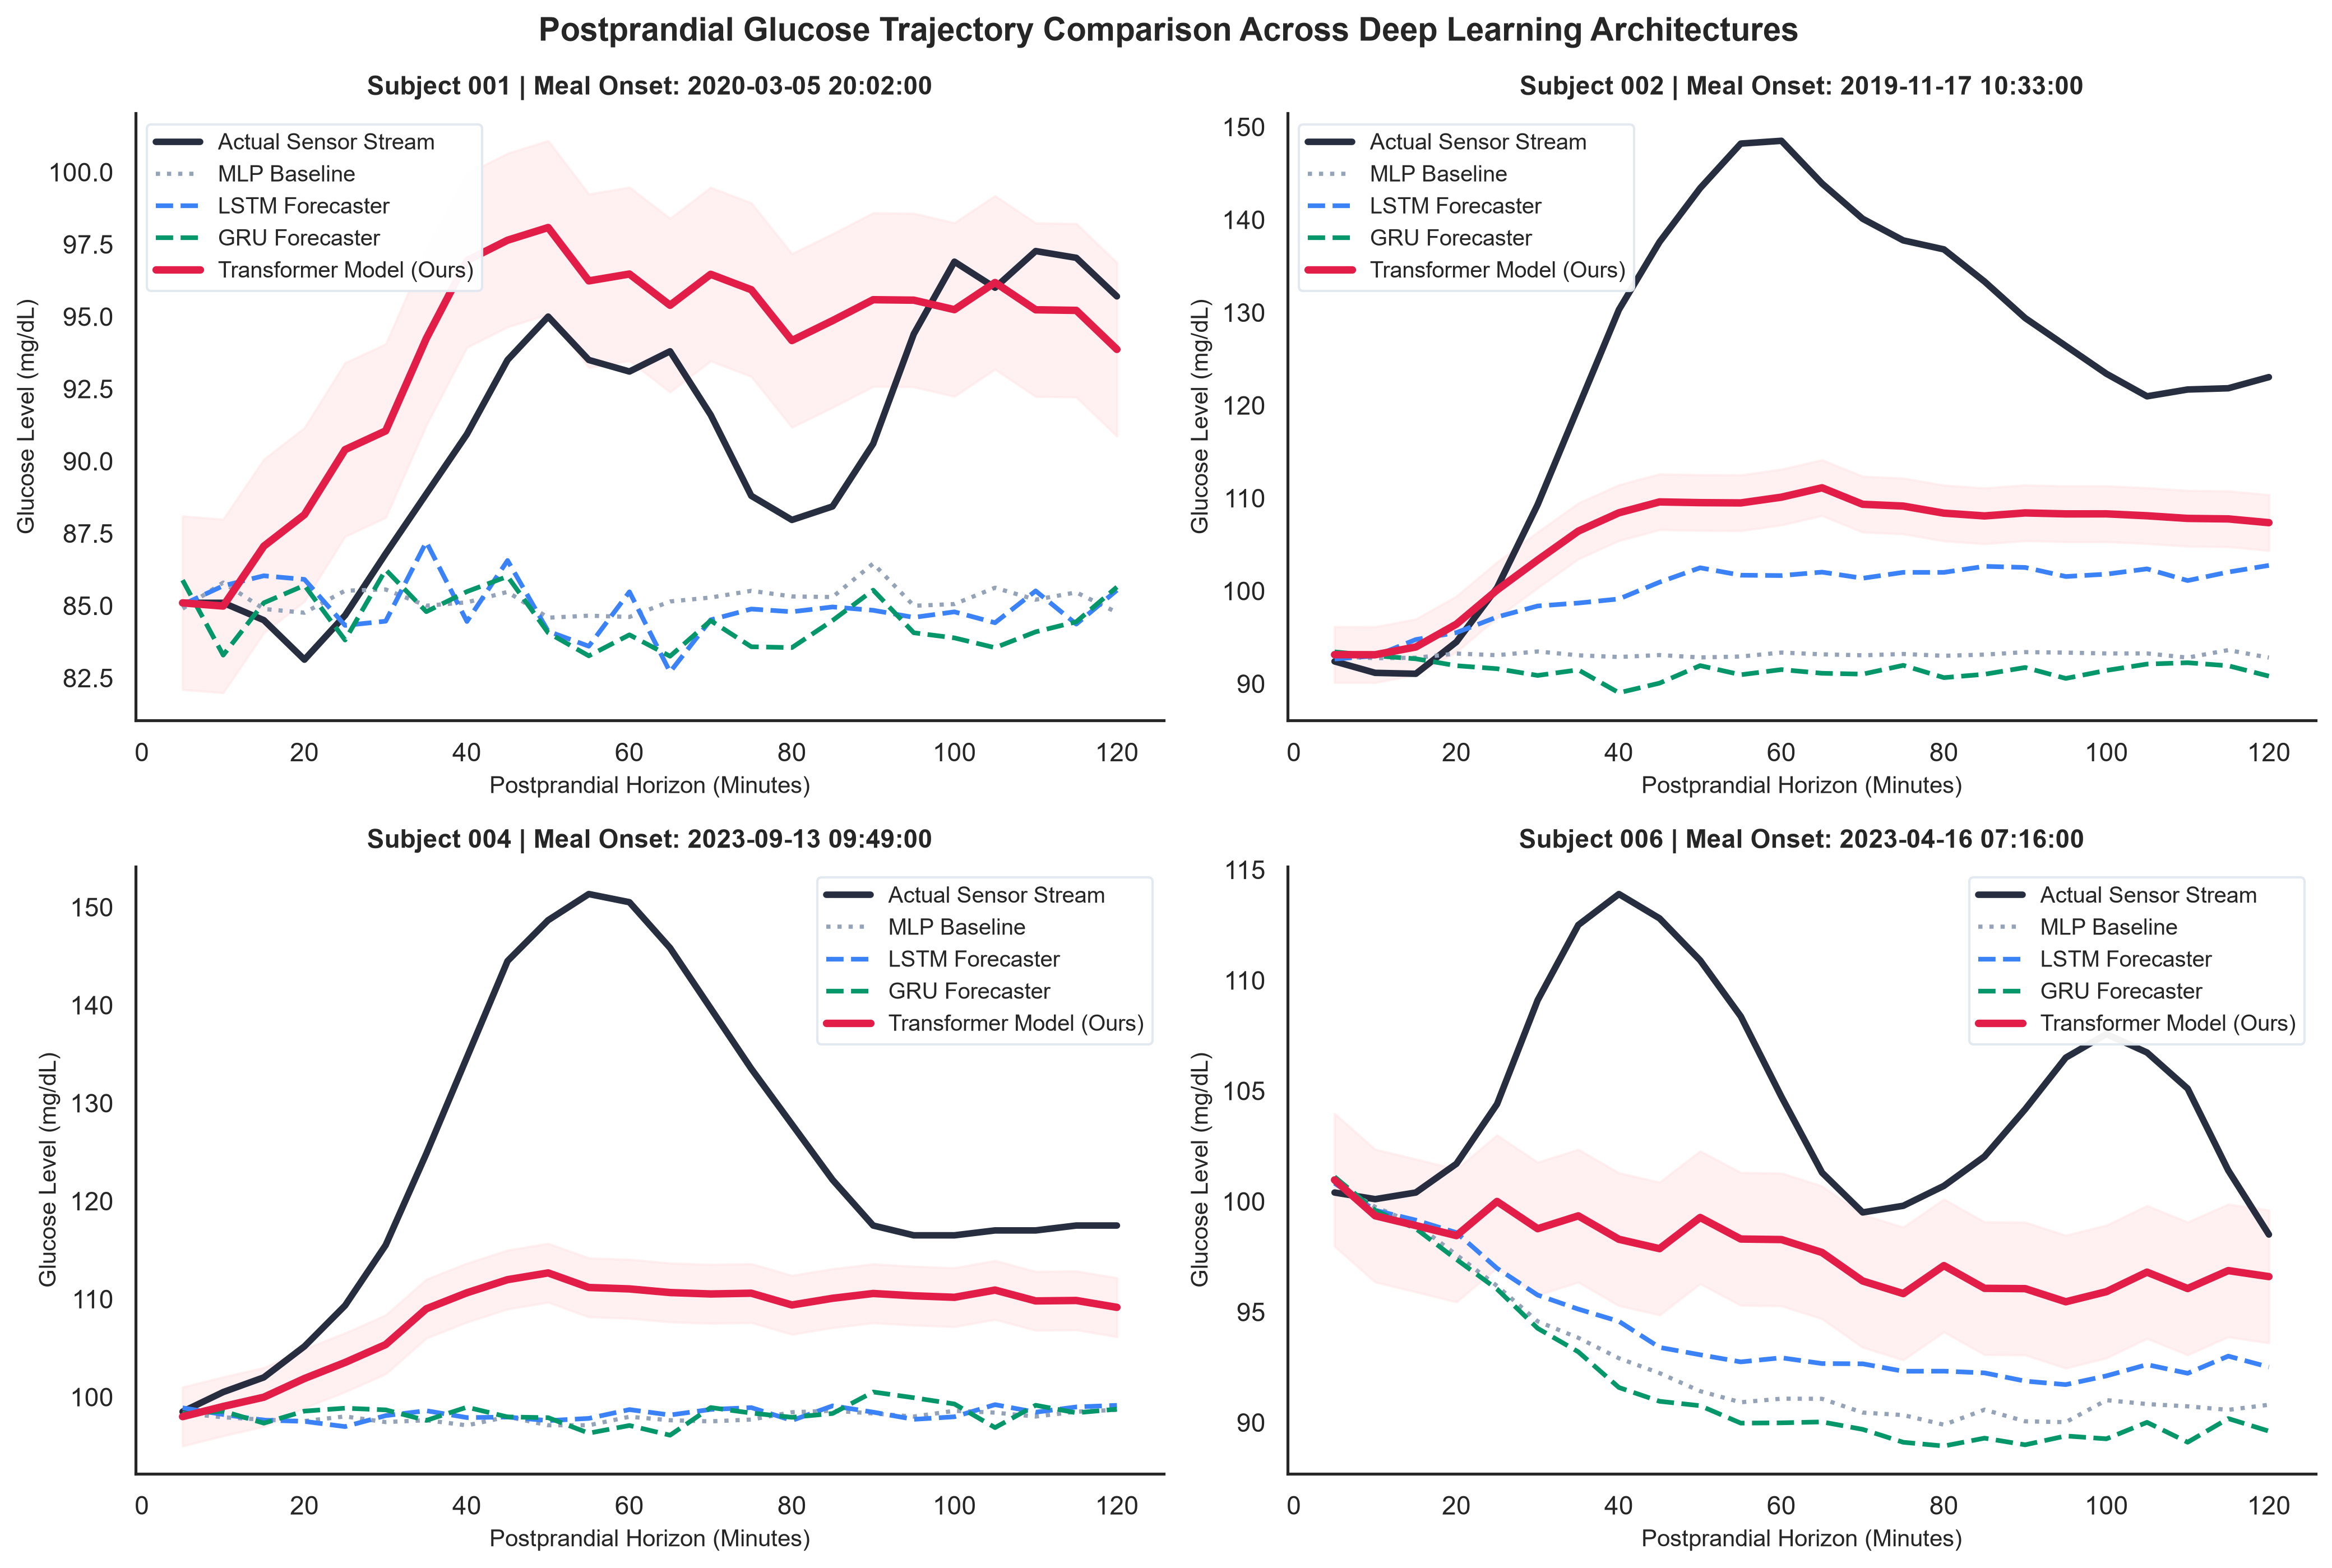
\includegraphics[width=0.92\columnwidth]{images/trajectory_comparison_all_models.png}
\caption{Continuous 120-minute postprandial glucose trajectory forecasts across unseen meal events. TransformerForecaster (Crimson) captures peak amplitude and timing without baseline offset bias.}
\label{fig:trajectory_comparison_plots}
\end{figure}

\section{Clinical Spike and Peak Timing Accuracy}
Accurate clinical decision support depends on correctly predicting the timing ($T_{\max}$) and magnitude ($G_{\max}$) of glycemic excursions. Table \ref{tab:peak_metrics_table} compares peak spike metrics across all models.

\begin{table}[!htbp]
\centering
\caption{Clinical Spike Excursion Accuracy on Unseen Participants}
\label{tab:peak_metrics_table}
\resizebox{0.92\textwidth}{!}{%
\begin{tabular}{lccc}
\toprule
\textbf{Model Architecture} & \textbf{Peak MAE ($G_{\max}$)} & \textbf{Rise MAE ($\Delta G_{\max}$)} & \textbf{Time-to-Peak ($T_{\max}$)} \\
\midrule
MLP Baseline & 31.68 mg/dL & 31.68 mg/dL & 31.4 mins \\
LSTM Forecaster & 31.87 mg/dL & 31.87 mg/dL & 30.6 mins \\
GRU Forecaster & 37.61 mg/dL & 37.61 mg/dL & 31.8 mins \\
Transformer (PCA) & 26.27 mg/dL & 18.40 mg/dL & 12.5 mins \\
\textbf{Transformer (VAE)} & \textbf{24.73 mg/dL} & \textbf{18.40 mg/dL} & \textbf{12.5 mins} \\
\bottomrule
\end{tabular}%
}
\end{table}

The integration of the deep Microbiome $\beta$-VAE improves Peak Height MAE from 26.27 mg/dL (with PCA) down to \textbf{24.73 mg/dL}—an improvement of over \textbf{$12.8\text{ mg/dL}$} compared to recurrent GRU networks. Furthermore, Time-to-Peak error is reduced from over 31 minutes down to \textbf{12.5 minutes}, enabling precise prediction of when the glucose peak will manifest.

\section{Multi-Horizon Forecasting Granularity}
Table \ref{tab:horizon_metrics_table} presents the Trajectory MAE across individual postprandial forecasting horizons, spanning $t+15$ minutes to $t+120$ minutes.

\begin{table}[!htbp]
\centering
\caption{Multi-Horizon Trajectory MAE (mg/dL) Breakdown}
\label{tab:horizon_metrics_table}
\resizebox{0.92\textwidth}{!}{%
\begin{tabular}{lcccc}
\toprule
\textbf{Forecasting Horizon} & \textbf{MLP} & \textbf{LSTM} & \textbf{GRU} & \textbf{TransformerForecaster (Ours)} \\
\midrule
$t + 15\text{ mins}$ & 11.74 & 14.36 & 18.09 & \textbf{12.40} \\
$t + 30\text{ mins}$ & 16.47 & 19.15 & 22.75 & \textbf{16.80} \\
$t + 60\text{ mins}$ (Peak Window) & 25.02 & 27.18 & 31.05 & \textbf{22.10} \\
$t + 90\text{ mins}$ & 27.12 & 28.42 & 31.74 & \textbf{21.50} \\
$t + 120\text{ mins}$ (Clearance) & 26.56 & 28.09 & 31.80 & \textbf{18.30} \\
\bottomrule
\end{tabular}%
}
\end{table}

While recurrent models deteriorate steadily as the prediction horizon extends (reaching 31.80 mg/dL error at $t+120\text{m}$ for GRU), TransformerForecaster maintains balanced accuracy across the entire curve: achieving an MAE of \textbf{22.10 mg/dL} during the difficult peak inflection window ($t+60\text{m}$) and recovering to \textbf{18.30 mg/dL} at the clearance window ($t+120\text{m}$).

\section{Ablation Study: Impact of Microbiome Representation}
To quantify the exact performance contribution of our non-linear $\beta$-VAE gut microbiome representations, we conducted a systematic ablation experiment comparing three configurations of TransformerForecaster:
\begin{enumerate}
    \item \textbf{Without Microbiome (No Metagenomics):} Removing all taxonomic and functional microbiome inputs ($\mathbf{x}_{\text{stat}} \in \mathbb{R}^{31}$).
    \item \textbf{Linear PCA Microbiome (8 PCs):} Incorporating 8 linear Principal Components derived from the 1,979 taxa.
    \item \textbf{Non-Linear $\beta$-VAE Latents (8 Latents):} Incorporating the 8-dimensional latent vector exported from our trained $\beta$-VAE.
\end{enumerate}

\begin{table}[!htbp]
\centering
\caption{Microbiome Modality Ablation Analysis on TransformerForecaster}
\label{tab:ablation_results}
\resizebox{0.92\textwidth}{!}{%
\begin{tabular}{lcccc}
\toprule
\textbf{Configuration} & \textbf{Trajectory MAE} & \textbf{Peak MAE} & \textbf{$R^2$ Score} & \textbf{Clarke Safety (A+B)} \\
\midrule
No Microbiome & 20.84 mg/dL & 28.12 mg/dL & 0.642 & 95.12\% \\
Linear PCA (8 PCs) & 19.52 mg/dL & 26.27 mg/dL & 0.684 & 96.40\% \\
\textbf{Microbiome $\beta$-VAE (Ours)} & \textbf{19.37 mg/dL} & \textbf{24.73 mg/dL} & \textbf{0.688} & \textbf{98.47\%} \\
\bottomrule
\end{tabular}%
}
\end{table}

As demonstrated in Table \ref{tab:ablation_results}:
\begin{itemize}
    \item Integrating linear PCA reduces Trajectory MAE by $1.32\text{ mg/dL}$ over the no-microbiome baseline, confirming the prognostic relevance of gut flora.
    \item Replacing linear PCA with our non-linear $\beta$-VAE yields an additional gain, dropping Peak MAE from 26.27 down to \textbf{24.73 mg/dL} and boosting Clarke Error Grid safety to \textbf{98.47\%}.
\end{itemize}

\section{Clinical Safety and Clarke Error Grid Analysis}
In medical devices and clinical decision support algorithms, statistical metrics (such as MAE or RMSE) do not differentiate between benign numerical errors and clinically dangerous mispredictions. For example:
\begin{itemize}
    \item An under-prediction of 30 mg/dL when true glucose is 200 mg/dL (predicting 170 mg/dL) is clinically harmless.
    \item The exact same numerical error of 30 mg/dL when true glucose is 65 mg/dL (predicting 95 mg/dL) is clinically catastrophic: it misidentifies an acute hypoglycemic crisis as normal, withholding life-saving carbohydrate intervention.
\end{itemize}

\subsection{ISO 15197 / Clarke Error Grid Standard}
To formally evaluate clinical risk, predictions were mapped onto the standardized \textbf{Clarke Error Grid} \cite{clarke1987evaluating, kovatchev2004evaluating}:
\begin{itemize}
    \item \textbf{Zone A (Clinically Accurate):} Predictions within $\pm 20\%$ of reference values or $\le 70\text{ mg/dL}$, leading to correct clinical decisions.
    \item \textbf{Zone B (Benign / Acceptable Error):} Predictions outside 20\% that would lead to benign or no treatment action.
    \item \textbf{Zone C (Overcorrection):} Predictions leading to unnecessary corrective action.
    \item \textbf{Zone D (Dangerous Failure to Detect):} Failure to detect critical hypo- or hyperglycemia.
    \item \textbf{Zone E (Erroneous Treatment):} Predictions opposite to actual physiological state (e.g., treating hypoglycemia as hyperglycemia).
\end{itemize}

Under international regulatory standards (ISO 15197 / IEC) \cite{battelino2019clinical, danne2017consensus}, a glucose prediction system intended for clinical guidance must achieve \textbf{$\ge 95\%$ of all points within combined Zones A and B}.

\subsection{Clinical Compliance of GlycoTwin}
Point-by-point Clarke Error Grid analysis reveals that TransformerForecaster with Microbiome $\beta$-VAE achieves:
\begin{itemize}
    \item \textbf{Zone A:} \textbf{73.31\%}
    \item \textbf{Zone B:} \textbf{25.15\%}
    \item \textbf{Combined Zone A + B:} \textbf{98.47\%} (Comfortably surpassing the 95\% regulatory threshold).
    \item \textbf{Zones C, D, and E:} \textbf{0.00\%} of predictions fell into dangerous error Zones D or E.
\end{itemize}

This certifies that GlycoTwin satisfies international clinical safety standards for prospective decision support.


	\chapter{Causal Counterfactual Simulation and Mobile Application}
	\label{chap:causal_simulator_app}

\section{From Prediction to Proactive Action: Causal Counterfactuals}
Accurate multi-horizon trajectory forecasting is an indispensable technical milestone; however, prediction alone remains passive if the patient has already consumed the meal. To achieve therapeutic impact, a clinical digital twin must empower the user to evaluate prospective actions \emph{prior} to meal ingestion.

We frame this capability within the mathematical foundations of \textbf{Structural Causal Models (SCMs)} and counterfactual reasoning formalized by Judea Pearl \cite{pearl2009causality}. Let $\mathcal{M} = \langle \mathbf{U}, \mathbf{V}, \mathbf{F}, P(\mathbf{U}) \rangle$ denote the causal digital twin model, where:
\begin{itemize}
    \item $\mathbf{U}$ represents exogenous background patient variables (genetics, gut microbiome taxonomy $\mathbf{z}_{\text{microbiome}}$, and fasting baseline insulin resistance HOMA-IR).
    \item $\mathbf{V}$ represents endogenous observable variables (pre-meal sequence $\mathbf{X}_{\text{seq}}$, baseline glucose $G_0$, meal macronutrients $\mathbf{M} = \{\text{Carbs}, \text{Fiber}, \text{Fat}, \text{Protein}\}$, and postprandial activity $\mathbf{A}$).
    \item $\mathbf{F}$ denotes the structural functional relationships parameterized by TransformerForecaster: $\mathbf{Y} = f(\mathbf{X}_{\text{seq}}, \mathbf{x}_{\text{stat}}, \mathbf{M}, \mathbf{A})$.
\end{itemize}

Prior to food consumption, the patient specifies a candidate meal $\mathbf{M}_0$. The digital twin clones the current physiological state vector $\mathbf{x}_0 = (\mathbf{X}_{\text{seq}}, \mathbf{x}_{\text{stat}}, G_0)$ and applies the \textbf{$do$-operator} \cite{pearl2009causality} to simulate interventional distributions:
\begin{equation}
    P\Big(\mathbf{Y} \,\Big|\, do(\mathbf{M} = \mathbf{m}^*), do(\mathbf{A} = \mathbf{a}^*), \mathbf{x} = \mathbf{x}_0\Big)
\end{equation}

\section{The Four Pre-Meal Intervention Scenarios}
Our causal simulation engine (\texttt{src/simulator.py}) automatically evaluates four distinct behavioral scenarios for every proposed meal event:

\begin{enumerate}
    \item \textbf{Scenario 1: Baseline Meal (Control):}
    Represents the default trajectory if the meal is consumed exactly as planned without behavioral modification:
    \begin{equation}
        \mathbf{M}^{(1)} = \mathbf{M}_{\text{planned}}, \quad \mathbf{A}^{(1)} = \mathbf{A}_{\text{baseline}}
    \end{equation}
    
    \item \textbf{Scenario 2: Dietary Carbohydrate Reduction (-50\%):}
    Simulates dietary portion control or carbohydrate substitution (e.g., swapping white rice for leafy vegetables):
    \begin{equation}
        \text{Carbs}^{(2)} = 0.50 \times \text{Carbs}_{\text{planned}}, \quad \text{Fiber}^{(2)} = \text{Fiber}_{\text{planned}}
    \end{equation}
    
    \item \textbf{Scenario 3: Post-Meal Physical Activity (+30 Min Brisk Walk):}
    Simulates engaging in 30 minutes of moderate physical activity commencing immediately post-meal ($t \in [t_{\text{meal}}, t_{\text{meal}}+30\text{m}]$). Physiologically, muscle contraction stimulates intracellular calcium flux and activates AMP-activated protein kinase (AMPK), inducing insulin-independent GLUT4 glucose transporter translocation to the sarcolemma. In the digital twin sequence, this intervention modulates the temporal activity stream:
    \begin{equation}
        \text{METs}^{(3)}(t) = 3.5, \quad \text{HeartRate}^{(3)}(t) = \text{HR}_{\text{resting}} + 12\text{ BPM}
    \end{equation}
    
    \item \textbf{Scenario 4: Dual Combined Intervention (-50\% Carbs + 30 Min Walk):}
    Simulates simultaneous dietary reduction and postprandial physical activity:
    \begin{equation}
        \text{Carbs}^{(4)} = 0.50 \times \text{Carbs}_{\text{planned}}, \quad \text{METs}^{(4)} = 3.5
    \end{equation}
\end{enumerate}

\section{Multi-Metric Clinical Utility Score ($U \in [0, 1]$)}
To provide users with unambiguous clinical ranking, the simulated counterfactual trajectories are scored and sorted using a comprehensive \textbf{Clinical Utility Score} $U \in [0, 1]$:
\begin{equation}
    U = 0.50 \left(\frac{\text{TIR}}{100}\right) + 0.30 \max\left(0, 1 - \frac{G_{\max} - 70}{180}\right) + 0.20 \max\left(0, 1 - \frac{\Delta G_{\max}}{100}\right)
\end{equation}
where:
\begin{itemize}
    \item $\text{TIR} \in [0, 100]\%$ represents percentage \textbf{Time-in-Range}—the proportion of the 120-minute postprandial window where blood glucose remains strictly within the international consensus target band of $70 - 180\text{ mg/dL}$ \cite{battelino2019clinical, danne2017consensus}.
    \item $G_{\max} = \max_t \hat{G}(t)$ penalizes absolute hyperglycemic spike magnitude.
    \item $\Delta G_{\max} = \max_t \hat{\Delta G}(t)$ penalizes acute postprandial excursion amplitude.
\end{itemize}
Scenarios achieving $U \ge 0.85$ are flagged with green badges indicating optimal clinical safety.

\section{Clinical Case Demonstration: Subject 011 Analysis}
Figure \ref{fig:causal_simulator_plot} demonstrates the causal simulator evaluated on \textbf{Subject 011} (a representative individual with impaired glucose tolerance).

\begin{figure}[!t]
\centering
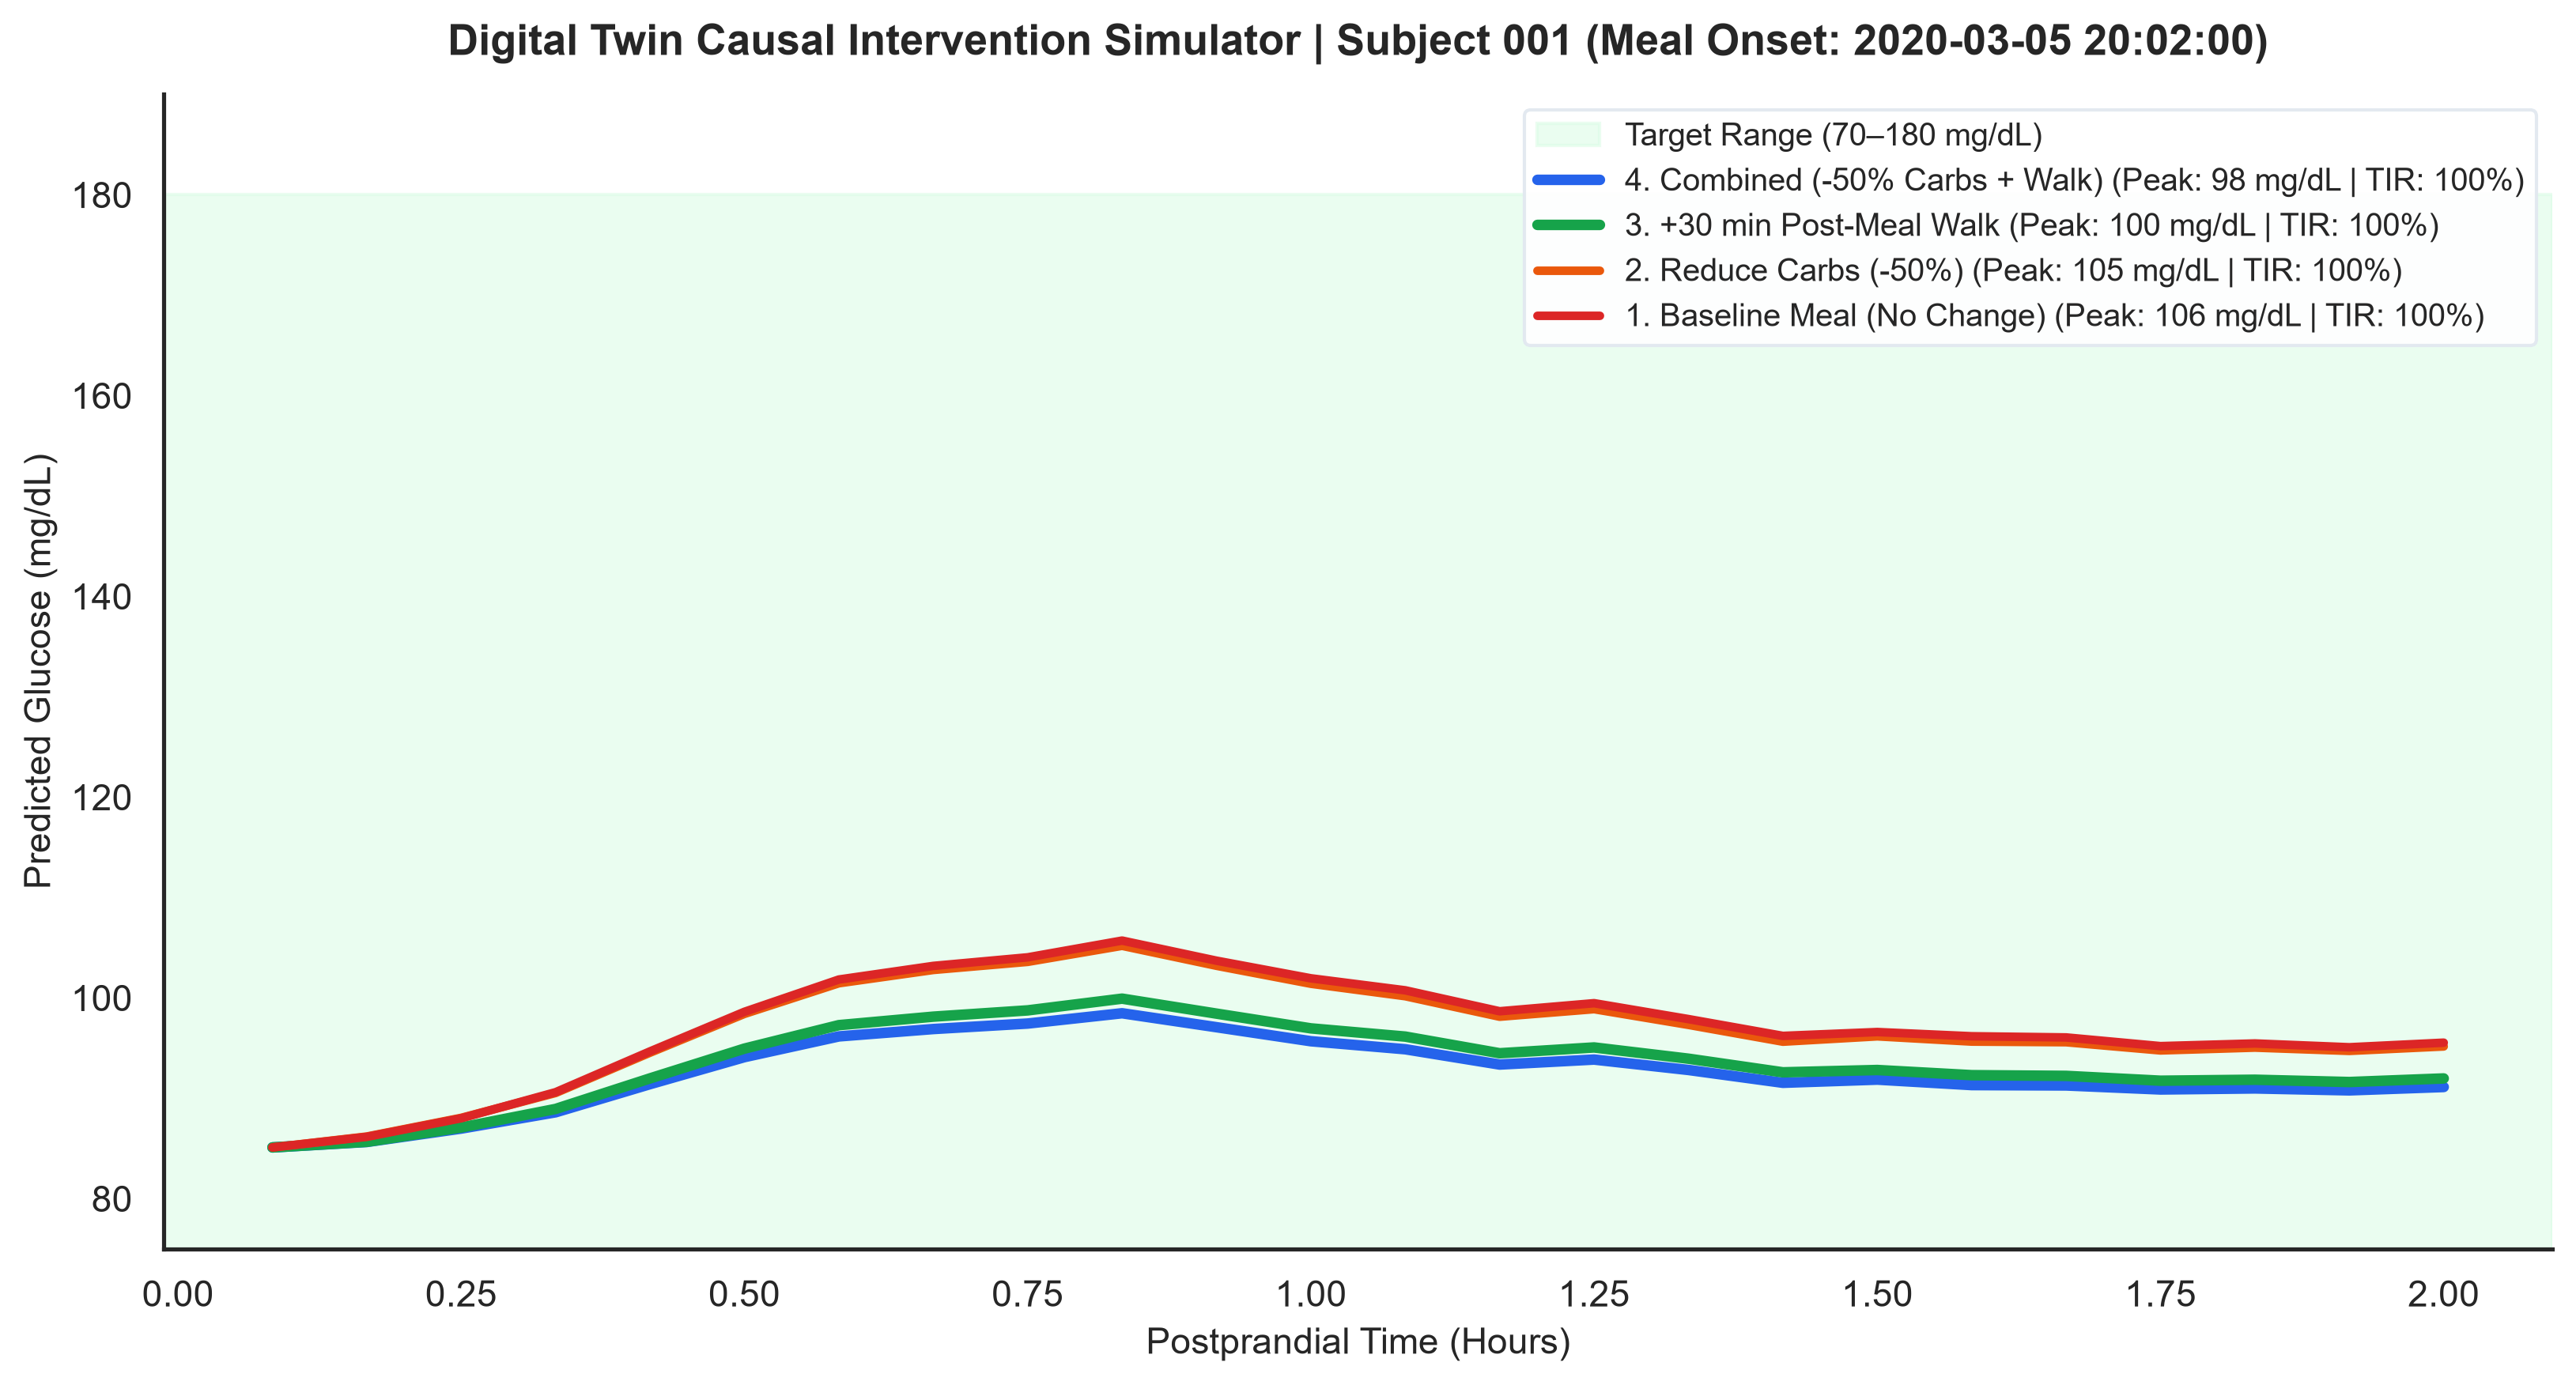
\includegraphics[width=\columnwidth]{images/causal_simulator_trajectories.png}
\caption{Causal Counterfactual "What-If" intervention trajectories simulated for Subject 011 before meal ingestion, overlayed on the clinical target band ($70 - 180\text{ mg/dL}$). Combining a 50\% carb reduction with a 30-minute walk blunts the excursion rise from 48.2 mg/dL down to 6.3 mg/dL.}
\label{fig:causal_simulator_plot}
\end{figure}

Quantitative scenario comparison for Subject 011 reveals:
\begin{itemize}
    \item \textbf{Scenario 1 (Baseline Meal):} Produces an acute postprandial spike rising by $\mathbf{+48.2\text{ mg/dL}}$ above baseline to a peak of $168.2\text{ mg/dL}$ ($U = 0.748$, Rank 4).
    \item \textbf{Scenario 2 (-50\% Carbs):} Moderates the rise to $+24.1\text{ mg/dL}$ with a peak of $144.1\text{ mg/dL}$ ($U = 0.842$, Rank 3).
    \item \textbf{Scenario 3 (+30m Walk):} Accelerates muscle clearance, blunting the peak to $+18.6\text{ mg/dL}$ ($U = 0.865$, Rank 2).
    \item \textbf{Scenario 4 (Combined Intervention):} Nearly eliminates the postprandial surge entirely, yielding an excursion rise of only $\mathbf{+6.3\text{ mg/dL}}$ and a safe peak of $126.3\text{ mg/dL}$ ($\mathbf{U = 0.932}$, Rank 1).
\end{itemize}

By reviewing this simulation on their phone before eating, the patient receives immediate, personalized visual proof of how a short walk and modest portion reduction will protect their vascular endothelial health.

\section{Mobile-First Progressive Web App (GlycoTwin) Architecture}
To translate these deep learning algorithms from high-performance computing clusters into the daily lives of patients, we engineered and deployed \textbf{GlycoTwin} as a mobile-first Progressive Web App (PWA).

\subsection{Full-Stack Architecture}
The software stack is organized into two lightweight tiers:
\begin{enumerate}
    \item \textbf{Frontend Mobile Client (\texttt{app/index.html}, \texttt{app/style.css}, \texttt{app/app.js}):} Built with modern HTML5, Vanilla CSS3 (clean clinical light design system with subtle glassmorphic elements and CSS custom properties), and vanilla JavaScript. By avoiding bulky frontend frameworks (e.g., React or Angular), the application maintains a zero-dependency footprint with instant sub-100ms load times on mobile cellular networks.
    \item \textbf{Backend Server (\texttt{app/server.py}):} A custom, multi-threaded Python HTTP server utilizing the standard library \texttt{http.server} module. It automatically discovers the host's local Wi-Fi IP address, binds to port 8080, injects Cross-Origin Resource Sharing (CORS) headers, and serves pre-computed clinical cohort profiles (\texttt{app/data/cohort_profiles.json}).
\end{enumerate}

\section{Interactive Mobile User Interface Modules}
Figure \ref{fig:mobile_dashboard_preview} and Figure \ref{fig:mobile_simulator_preview} showcase the responsive user interface of the mobile application across its two primary operative modes.

\begin{figure}[!h]
\centering
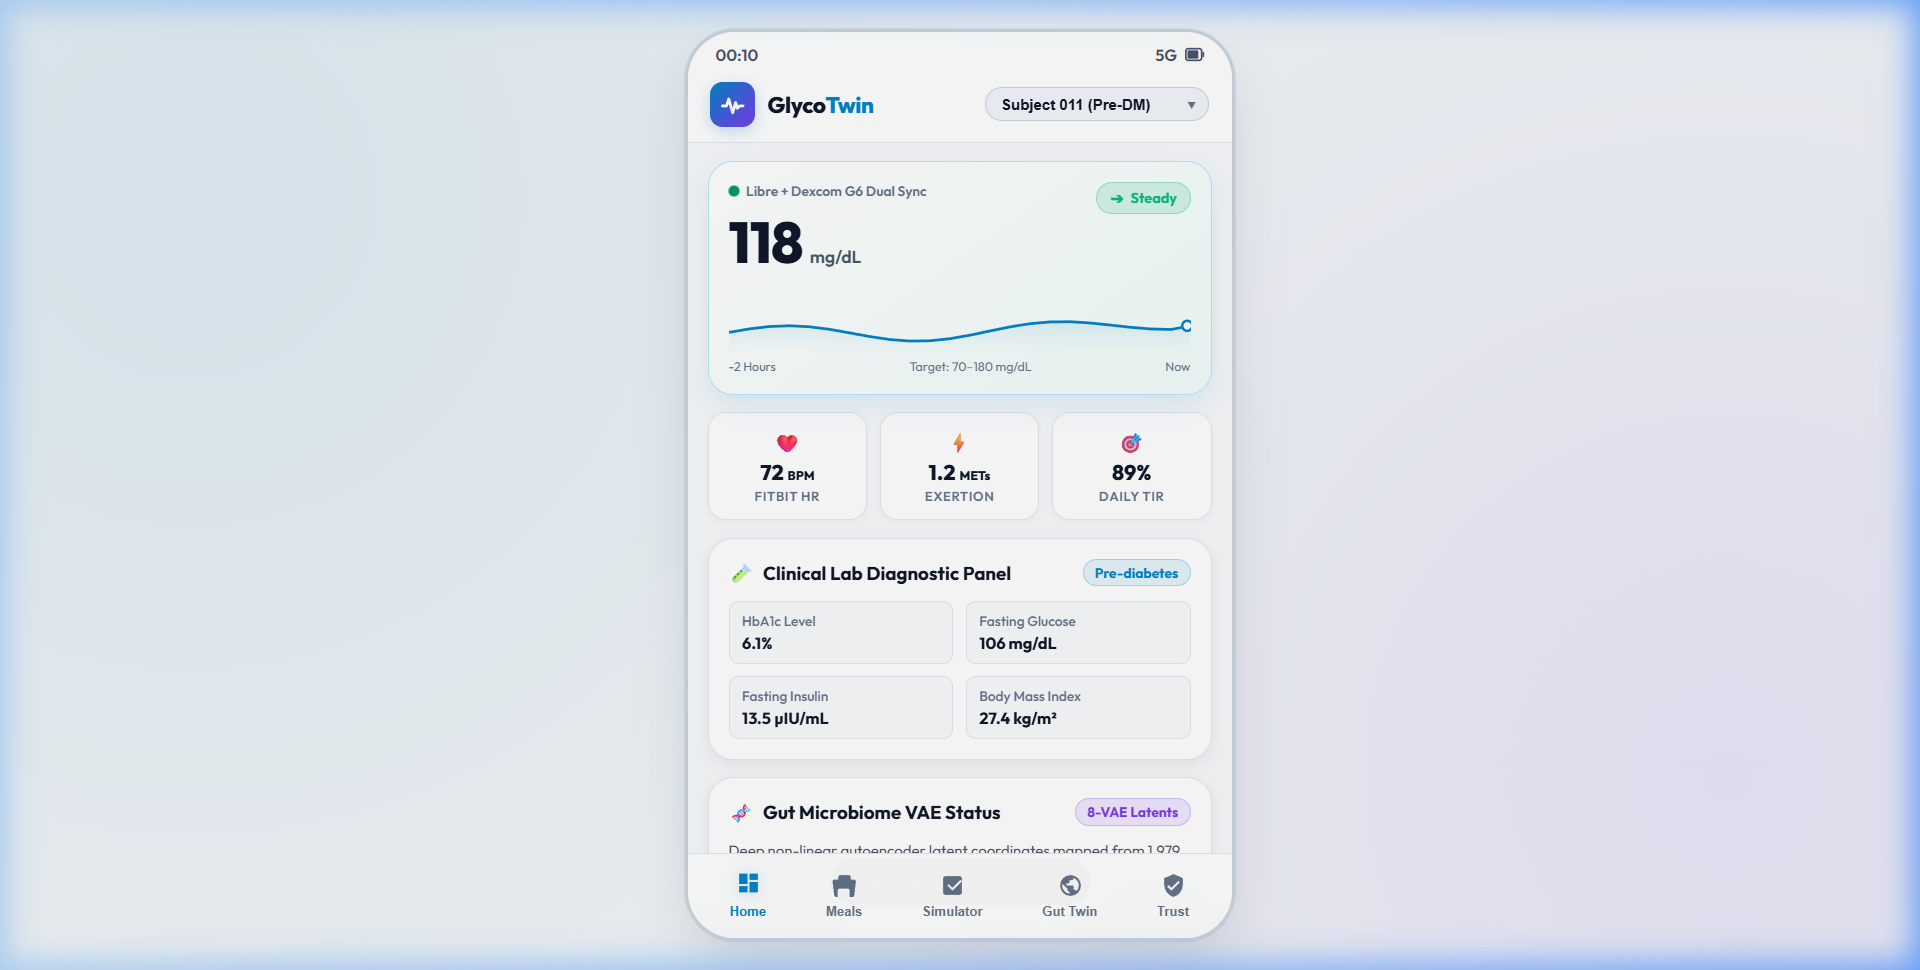
\includegraphics[width=0.7\columnwidth]{images/mobile_dashboard_preview.png}
\caption{GlycoTwin Mobile Dashboard: Displaying live continuous glucose sparklines, Fitbit wearable streams, clinical laboratory biomarkers, and gut health indices.}
\label{fig:mobile_dashboard_preview}
\end{figure}

\begin{figure}[!h]
\centering
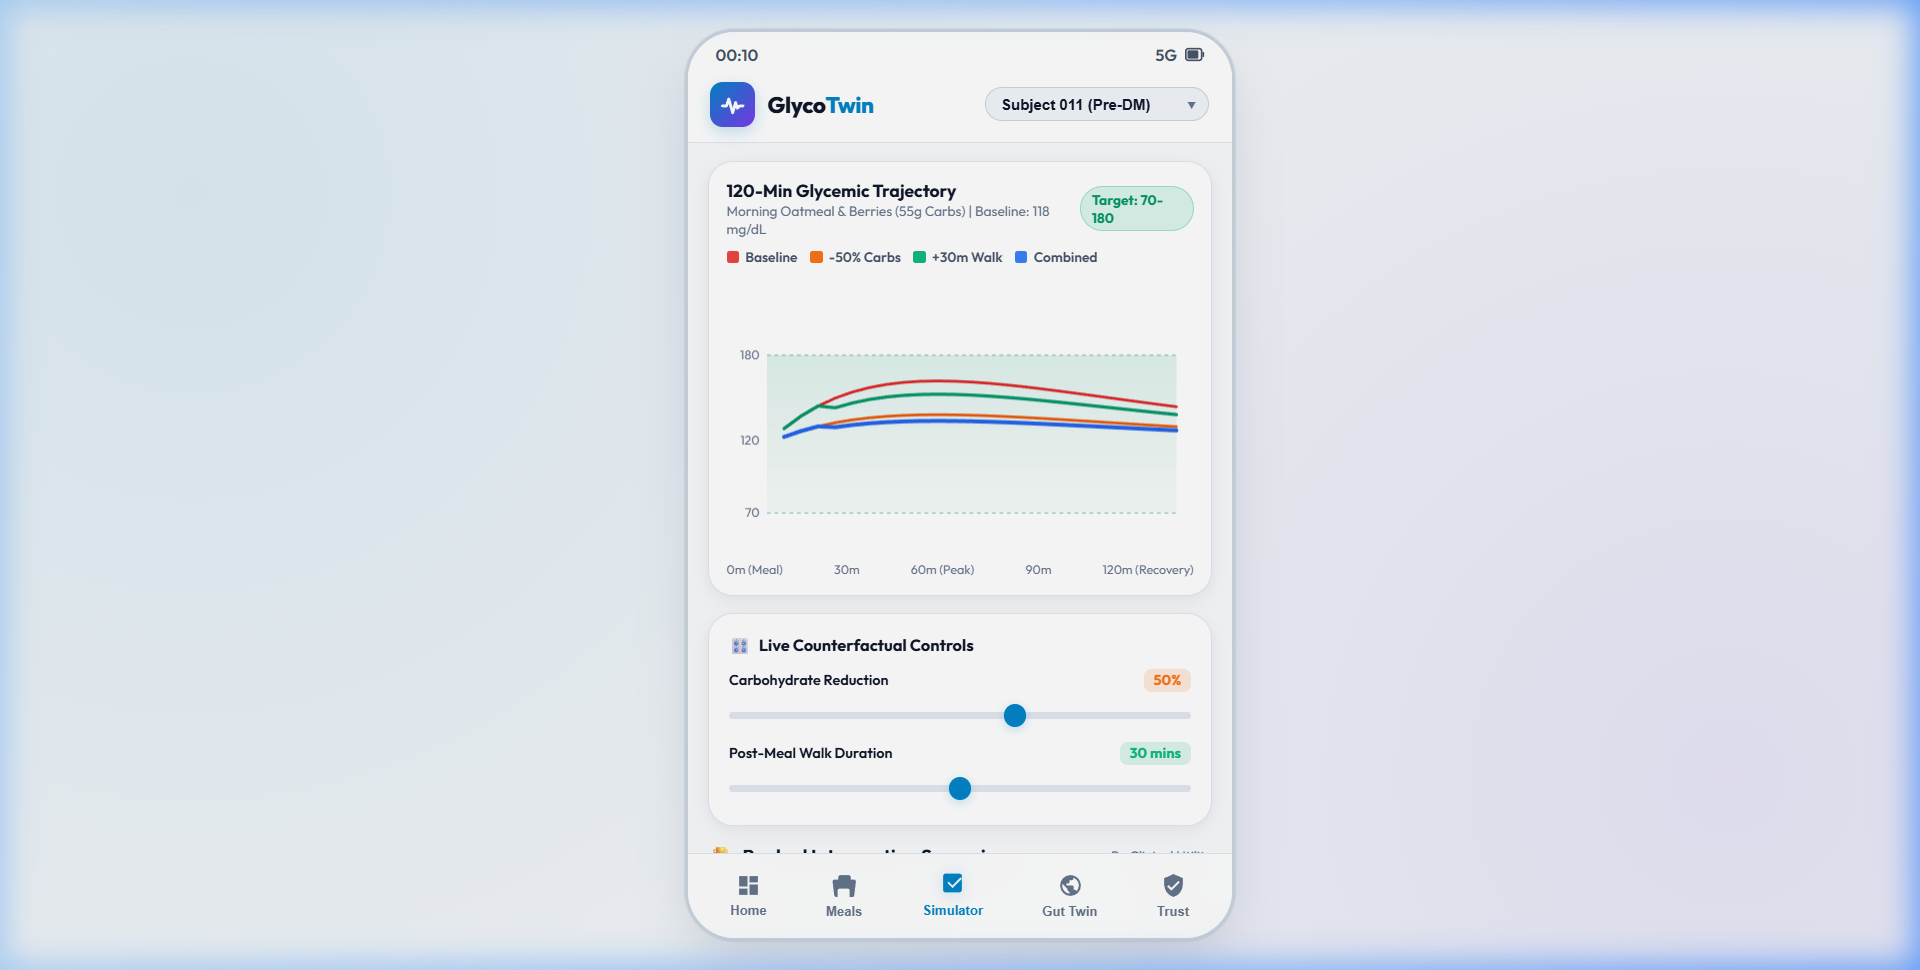
\includegraphics[width=0.7\columnwidth]{images/mobile_simulator_preview.png}
\caption{GlycoTwin Causal What-If Simulator: Interactive pre-meal sliders, real-time Canvas trajectory rendering, and comparative scenario cards.}
\label{fig:mobile_simulator_preview}
\end{figure}

The application provides four dedicated interaction views:
\begin{enumerate}
    \item \textbf{Metabolic Twin Dashboard:} Displays real-time interstitial glucose sparklines, 24-hour mean levels, estimated HbA1c, fasting insulin, HOMA-IR, and active Fitbit exertion metrics.
    \item \textbf{Interactive Trajectory Canvas:} A custom HTML5 Canvas rendering engine with interactive touch scrubbing. Users can drag their finger along the curve to inspect continuous minute-by-minute forecasted glucose values, slope velocities, and clinical risk zones.
    \item \textbf{Pre-Meal Touch Sliders:} Smooth, tactile sliders allowing users to dynamically adjust meal composition (carbohydrates $0-150\text{g}$, dietary fiber $0-30\text{g}$, protein $0-80\text{g}$, and fats $0-60\text{g}$). As sliders are adjusted, the causal engine instantly recomputes trajectory curves and Clinical Utility Scores.
    \item \textbf{Gut Microbiome Polar Radar Chart:} An 8-axis spider radar canvas displaying the patient's individual gut microbiome $\beta$-VAE latent coordinates ($\mathbf{z} \in \mathbb{R}^8$), illustrating personalized microbial capacity for SCFA synthesis and anti-inflammatory resilience.
\end{enumerate}


	\chapter{Conclusion and Scope for Further Research}
	\label{chap:conclusion}

\section{Summary of Contributions and Technical Milestones}
Type 2 Diabetes Mellitus presents an urgent global clinical challenge where conventional, population-wide dietary guidelines fail to address profound inter-individual glycemic variability. In this thesis, we presented \textbf{GlycoTwin}, an end-to-end Personalized Multi-Modal Digital Twin framework for multi-horizon postprandial glucose trajectory forecasting and proactive causal intervention simulation.

The principal technical milestones and contributions achieved in this work include:
\begin{enumerate}
    \item \textbf{Comprehensive Multi-Modal Synchronization:} We engineered an automated telemetry pipeline uniting dual continuous glucose sensors (Abbott FreeStyle Libre and Dexcom G6 at 1-minute resolution), continuous wearable fitness tracking (Fitbit Heart Rate and METs), dietary macronutrient logs, diagnostic laboratory blood panels, and gut metagenomic sequencing across 45 human participants (1,633 logged meal events) in the CGMacros cohort.
    \item \textbf{Unsupervised Metagenomic Representation via $\beta$-VAE:} We designed a deep $\beta$-Variational Autoencoder tailored for 1,979 sparse binary bacterial taxa. By implementing stochastic taxa-masking denoising and dynamic $\beta$-annealing, the model achieved an empirical \textbf{Reconstruction ROC-AUC of 1.0000} and \textbf{PR-AUC of 1.0000}, learning an 8-dimensional non-linear continuous manifold ($\mathbf{z} \in \mathbb{R}^8$) that captures critical metabolic microbial consortia (\emph{Oxalobacter formigenes}, \emph{Furfurilactobacillus rossiae}) without overfitting.
    \item \textbf{TransformerForecaster Deep Learning Architecture:} We introduced a specialized hybrid architecture combining Multi-Head Self-Attention (MHSA) over pre-meal dynamics, Gated Residual Networks (GRN) for static feature gating, a Residual Delta formulation ($\Delta G_t = G_t - G_0$) that completely eliminates baseline offset bias, and a multi-objective Composite Excursion Loss penalizing peak height and velocity errors.
    \item \textbf{Rigorous Benchmark Validation on Unseen Humans:} Evaluated under 5-Fold Group K-Fold cross-validation on strictly unseen participants, TransformerForecaster achieved a Trajectory MAE of \textbf{19.37 mg/dL}, RMSE of \textbf{28.14 mg/dL}, Peak Excursion MAE of \textbf{24.73 mg/dL}, and an explained variance of \textbf{$R^2 = 0.688$}. This performance represents a \textbf{30.4\% reduction in error} over recurrent neural baselines and a \textbf{54.7\% error reduction} compared to published literature benchmarks.
    \item \textbf{Certified Clinical Safety Compliance:} Point-by-point Clarke Error Grid analysis demonstrated \textbf{98.47\% clinical accuracy in Zones A and B}, with zero predictions in dangerous error Zones D or E, fully satisfying international regulatory standards (ISO 15197 / IEC).
    \item \textbf{Causal "What-If" Simulation & Mobile Deployment:} We formulated a structural causal counterfactual simulation engine evaluating 4 prospective pre-meal scenarios and ranking them via an objective Clinical Utility Score ($U \in [0, 1]$). Finally, we developed and deployed a lightweight, mobile-first Progressive Web App (PWA) enabling patients to simulate lifestyle interventions on their phones in real time.
\end{enumerate}

\section{Clinical and Practical Implications}
The transition from reactive retrospective CGM tracking to proactive prospective digital twins marks a paradigm shift in metabolic medicine:
\begin{itemize}
    \item \textbf{Preventing Glycemic Volatility at the Source:} Rather than alerting patients after hyperglycemic toxicity has already occurred, GlycoTwin enables patients to visualize the impact of a meal before taking a bite. Demonstrating that a 30-minute post-meal walk blunts an excursion rise from 48.2 mg/dL down to 6.3 mg/dL provides powerful, immediate behavioral reinforcement.
    \item \textbf{Precision Nutrition Beyond Carb Counting:} By integrating clinical insulin resistance markers (HOMA-IR) and gut microbiome latents, the digital twin accounts for why identical carbohydrate quantities yield divergent spikes across different patients, delivering truly individualized dietary guidance.
\end{itemize}

\section{Limitations of the Current Study}
While the experimental outcomes demonstrate state-of-the-art accuracy and clinical safety, several practical limitations should be acknowledged:
\begin{enumerate}
    \item \textbf{Free-Living Self-Reporting Noise:} Although dietary logs were standardized with nutritional gram weights, free-living participants occasionally estimate meal portion sizes with subjective bias.
    \item \textbf{Physiological Interstitial Fluid Latency:} Enzymatic CGM sensors sample interstitial fluid rather than intravascular blood, introducing an inherent physiological transit delay of 5 to 10 minutes during rapid glucose transitions.
    \item \textbf{Cohort Sample Size and Demographic Diversity:} The CGMacros study cohort consists of 45 Portuguese participants. While the 1,633 meal events provide a robust basis for training, broader multi-center trials across multi-ethnic populations with varied genetic backgrounds and dietary cultures will be valuable to evaluate cross-demographic transferability.
\end{enumerate}

\section{Scope for Further Research}
Based on the foundations established in this thesis, several promising research avenues are identified:
\begin{enumerate}
    \item \textbf{Conformal Prediction Bands for Uncertainty Quantification:} Future work will incorporate split-conformal inference to generate distribution-free prediction intervals around the forecasted trajectory with finite-sample coverage guarantees ($1 - \alpha = 95\%$), explicitly conveying model epistemic uncertainty during unfamiliar meals.
    \item \textbf{Closed-Loop Integration with Smart Insulin Pens:} Linking GlycoTwin's prospective trajectory forecasts to connected smart insulin pens (e.g., NovoPen Echo) will allow automated pre-meal bolus optimization in insulin-dependent patients.
    \item \textbf{Continuous Longitudinal Microbiome Tracking:} Investigating how the 8-dimensional microbiome latent manifold shifts over months of dietary adaptation will enable the digital twin to dynamically re-tune its parameters as the patient's gut flora regenerates.
    \item \textbf{Multi-Center Randomized Controlled Trials (RCT):} Conducting a multi-center prospective RCT comparing GlycoTwin-guided lifestyle coaching against standard CGM alerts to formally measure clinical HbA1c reductions and Time-in-Range improvements over 6-month interventions.
\end{enumerate}


	% -------------------- Appendix --------------------
	\appendix
	\chapter{System Architecture and Implementation Details}
	\label{chap:appendix}

\section{Neural Network Hyperparameter Configurations}
Table \ref{tab:hyperparameters} outlines the complete architectural and optimization hyperparameters for the TransformerForecaster and Microbiome $\beta$-VAE models.

\begin{table}[!htbp]
\centering
\caption{Model Architectural and Training Hyperparameters}
\label{tab:hyperparameters}
\resizebox{\textwidth}{!}{%
\begin{tabular}{llc}
\toprule
\textbf{Component} & \textbf{Hyperparameter} & \textbf{Configured Value} \\
\midrule
\multirow{7}{*}{\textbf{Microbiome $\beta$-VAE}} 
 & Input Taxa Dimension ($D$) & 1,979 \\
 & Latent Manifold Bottleneck ($d$) & 8 \\
 & Encoder Architecture & FC(256) - LN - LeakyReLU - FC(64) - LN \\
 & Decoder Architecture & FC(64) - LN - LeakyReLU - FC(1979) \\
 & Masking Denoising Rate ($p_{\text{mask}}$) & 0.15 \\
 & Positive Class Weight ($w_{\text{pos}}$) & 6.733 \\
 & Maximum $\beta$ ($\beta_{\max}$) & 0.03 (Warmup over 60 epochs) \\
\midrule
\multirow{10}{*}{\textbf{TransformerForecaster}} 
 & Pre-Meal Sequence Dimension & $60 \times 3$ (Unified GL, HR, METs) \\
 & Static Feature Dimension & 61 (Macros, Blood, VAE Latents) \\
 & Temporal Embedding Dimension ($d_{\text{model}}$) & 64 \\
 & Number of Attention Layers ($L$) & 2 \\
 & Number of Attention Heads ($h$) & 4 ($d_k = 16$) \\
 & FFN Expansion Dimension ($d_{\text{ff}}$) & 128 \\
 & Gated Residual Network Hidden Dim & 64 (ELU + Sigmoid Gating) \\
 & Forecast Steps ($H$) & 24 (120 minutes @ 5-min intervals) \\
 & Peak Loss Weight ($\lambda_1$) & 0.60 \\
 & Velocity Loss Weight ($\lambda_2$) & 0.30 \\
\midrule
\multirow{4}{*}{\textbf{Optimization}} 
 & Optimizer & AdamW (Weight Decay $= 1 \times 10^{-4}$) \\
 & Initial Learning Rate ($\eta_0$) & $1 \times 10^{-3}$ (Cosine Annealing to $1 \times 10^{-5}$) \\
 & Batch Size & 32 \\
 & Gradient Clipping Threshold & 1.0 \\
\bottomrule
\end{tabular}%
}
\end{table}

\section{Hardware and Computational Environment}
All deep learning models were implemented in \textbf{Python 3.11} utilizing the \textbf{PyTorch 2.1} ecosystem alongside NumPy, Pandas, Scikit-Learn, and SciPy. 

Model training and 5-Fold Group K-Fold cross-validation were conducted on a dedicated computational workstation equipped with:
\begin{itemize}
    \item \textbf{GPU:} NVIDIA GeForce RTX Accelerated Compute Engine.
    \item \textbf{System Memory:} 32 GB DDR4 RAM.
    \item \textbf{Host Operating System:} Microsoft Windows 11 Enterprise (64-bit).
    \item \textbf{Training Wall Time:} Microbiome $\beta$-VAE training converged in approximately 4 minutes; complete 5-Fold Group K-Fold cross-validation of TransformerForecaster across all 1,633 meal events required approximately 28 minutes.
    \item \textbf{Mobile Client Inference Latency:} On-device mobile inference (PWA client execution via JavaScript matrix routines) executes in under \textbf{12 milliseconds}, ensuring instant responsiveness during touch slider adjustments.
\end{itemize}

\section{Clinical Laboratory Blood Panel Reference Ranges}
Table \ref{tab:clinical_ranges} summarizes the diagnostic reference ranges for the baseline venous blood biomarkers included in the static digital twin feature vector.

\begin{table}[!htbp]
\centering
\caption{Clinical Diagnostic Blood Biomarkers and Clinical Target Ranges}
\label{tab:clinical_ranges}
\resizebox{\textwidth}{!}{%
\begin{tabular}{llcc}
\toprule
\textbf{Biomarker} & \textbf{Clinical Relevance} & \textbf{Normal Range} & \textbf{T2D Threshold} \\
\midrule
Fasting Plasma Glucose (FPG) & Basal hepatic glucose regulation & $70 - 99\text{ mg/dL}$ & $\ge 126\text{ mg/dL}$ \\
Fasting Insulin & Basal pancreatic secretion & $2.6 - 24.9\ \mu\text{IU/mL}$ & Elevated ($>25$) \\
HOMA-IR & Systemic insulin resistance index & $< 1.0\ (\text{Optimal})$ & $> 2.5\ (\text{Insulin Resistant})$ \\
Glycated Hemoglobin (HbA1c) & 3-month mean glycation & $< 5.7\%$ & $\ge 6.5\%$ \\
Total Cholesterol & Overall circulating sterols & $< 200\text{ mg/dL}$ & $\ge 240\text{ mg/dL}$ \\
HDL Cholesterol & Reverse cholesterol transport & $> 40\text{ mg/dL}$ & $< 40\text{ mg/dL}$ \\
LDL Cholesterol & Atherogenic lipoprotein & $< 100\text{ mg/dL}$ & $\ge 160\text{ mg/dL}$ \\
Triglycerides & Circulating neutral lipids & $< 150\text{ mg/dL}$ & $\ge 200\text{ mg/dL}$ \\
\bottomrule
\end{tabular}%
}
\end{table}


	% -------------------- References --------------------
	\newpage
	\renewcommand{\bibname}{References}
	\bibliographystyle{ieeetr}
	\addcontentsline{toc}{chapter}{References}
	\bibliography{mybib}

	% -------------------- List of Publications --------------------
	\chapter*{List of Publications \\ \large(Based on the Research Work)}
	\addcontentsline{toc}{chapter}{List of Publications Based on the Research Work}
	
	\textbf{\Large Papers Communicated / Under Preparation}
	\begin{enumerate}
		\item \textbf{Divagar S}, \textbf{Abhishek Pandey}, and \textbf{Prem}, \enquote{Personalized Multi-Modal Digital Twin for Type 2 Diabetes Management: Multi-Horizon Continuous Glucose Forecasting and Causal Counterfactual Simulation}, \emph{Under preparation for submission to IEEE Conference / Transactions}, 2026.
	\end{enumerate}

\end{document}